\documentclass{beamer}

\beamertemplatenavigationsymbolsempty
\usepackage{gensymb}
\usepackage[utf8]{inputenc}
\usepackage{xspace}
\usepackage{siunitx}
\usepackage{bm}
\graphicspath{ {./graphics/} }
\usepackage{amssymb}
\usepackage{amsmath}
\usepackage{amsfonts}
\usepackage{color}
\usepackage{isotope}

\definecolor{mypurple}{RGB}{128, 0, 128}

\newcommand{\be}{$\beta$}
\newcommand{\al}{$\alpha$}
\newcommand{\li}{\isotope[8]{Li}\xspace}
\newcommand{\ber}{\isotope[8]{Be}\xspace}


%Information to be included in the title page:
\title{Speciale Forsvar}
\subtitle{Studying the angular correlation and final state distribution in the $^8$Li beta-decay }
\author{Anders Holst Rasmussen}
\date{28. Juni, 2021}

\mode<presentation> {
	\usetheme{CambridgeUS}
	\usecolortheme{seahorse}
	%\setbeamercovered{transparent}
}

\AtBeginSection[]
{
	\begin{frame}
		\frametitle{Oversigt}
		\tableofcontents[currentsection]
	\end{frame}
}

\begin{document}
\frame\titlepage
\section{Introduktion}

\begin{frame}{\be-henfald}
	To typer:
	\begin{align*}
	\onslide<2->{&\beta^+:\quad p\rightarrow n + e^+ + \nu_e\\}
	\onslide<2->{&\beta^-:\quad n\rightarrow p + e^- + \bar{\nu_e}}
	\end{align*}
	\onslide<3->{Forskellige Q-værdier:}
	\begin{align*}
	\onslide<4->{&Q_{\beta^+} = \left[ m (\isotope[A][Z]{X}) - m(\isotope[A][Z-1]{X'})  		 \right] c^2\\
	&Q_{\beta^-} = \left[ m (\isotope[A][Z]{X}) - m(\isotope[A][Z+1]{X'}) -2m_e  \right] c^2}
	\end{align*}
\end{frame}

\begin{frame}{\be-henfald}
	Tilladte overgange:
	\begin{equation*}
	\onslide<2->{\Delta J = 0, \pm1,\ \Delta T = 0, \pm 1,\ \text{og}\ \Delta \pi = 0}
	\end{equation*}
	\onslide<3->{Spin, paritiet og isospin: $J^\pi ; T$}
	\onslide<4->{
		\begin{figure}
			\centering
			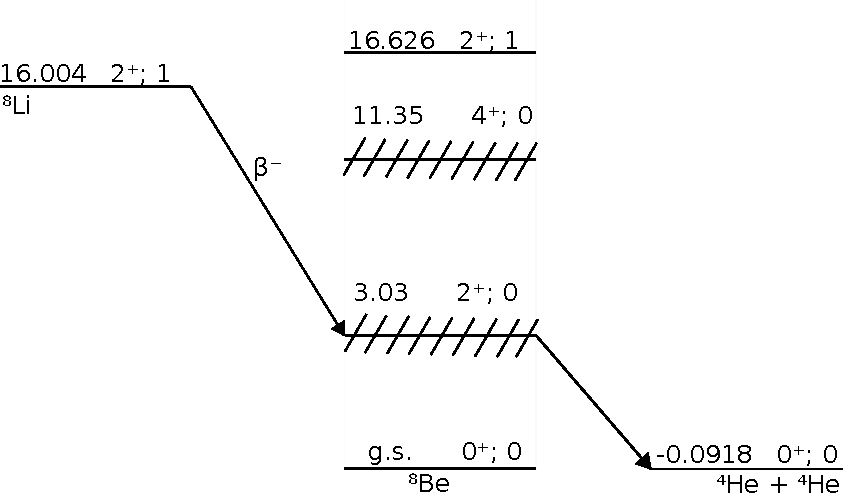
\includegraphics[width=.6\columnwidth]{../figures/DecayScheme.pdf}
		\end{figure}
	}
\end{frame}

\begin{frame}{\al-henfald}
	Udsendelsen af \al-partikel\\
	\onslide<2->{Q-værdi:
		\begin{equation*}
			Q_\alpha = \left[ m\left(^A_Z X\right) - m\left( ^{A-4}_{Z-2} X' \right) -m_\alpha \right]c^2
		\end{equation*}
	}
\end{frame}
\section{Eksperimentel opsætning}

\begin{frame}{Eksperimentel opsætning}
	\begin{columns}
		\column{0.4\textwidth}
		\begin{figure}
			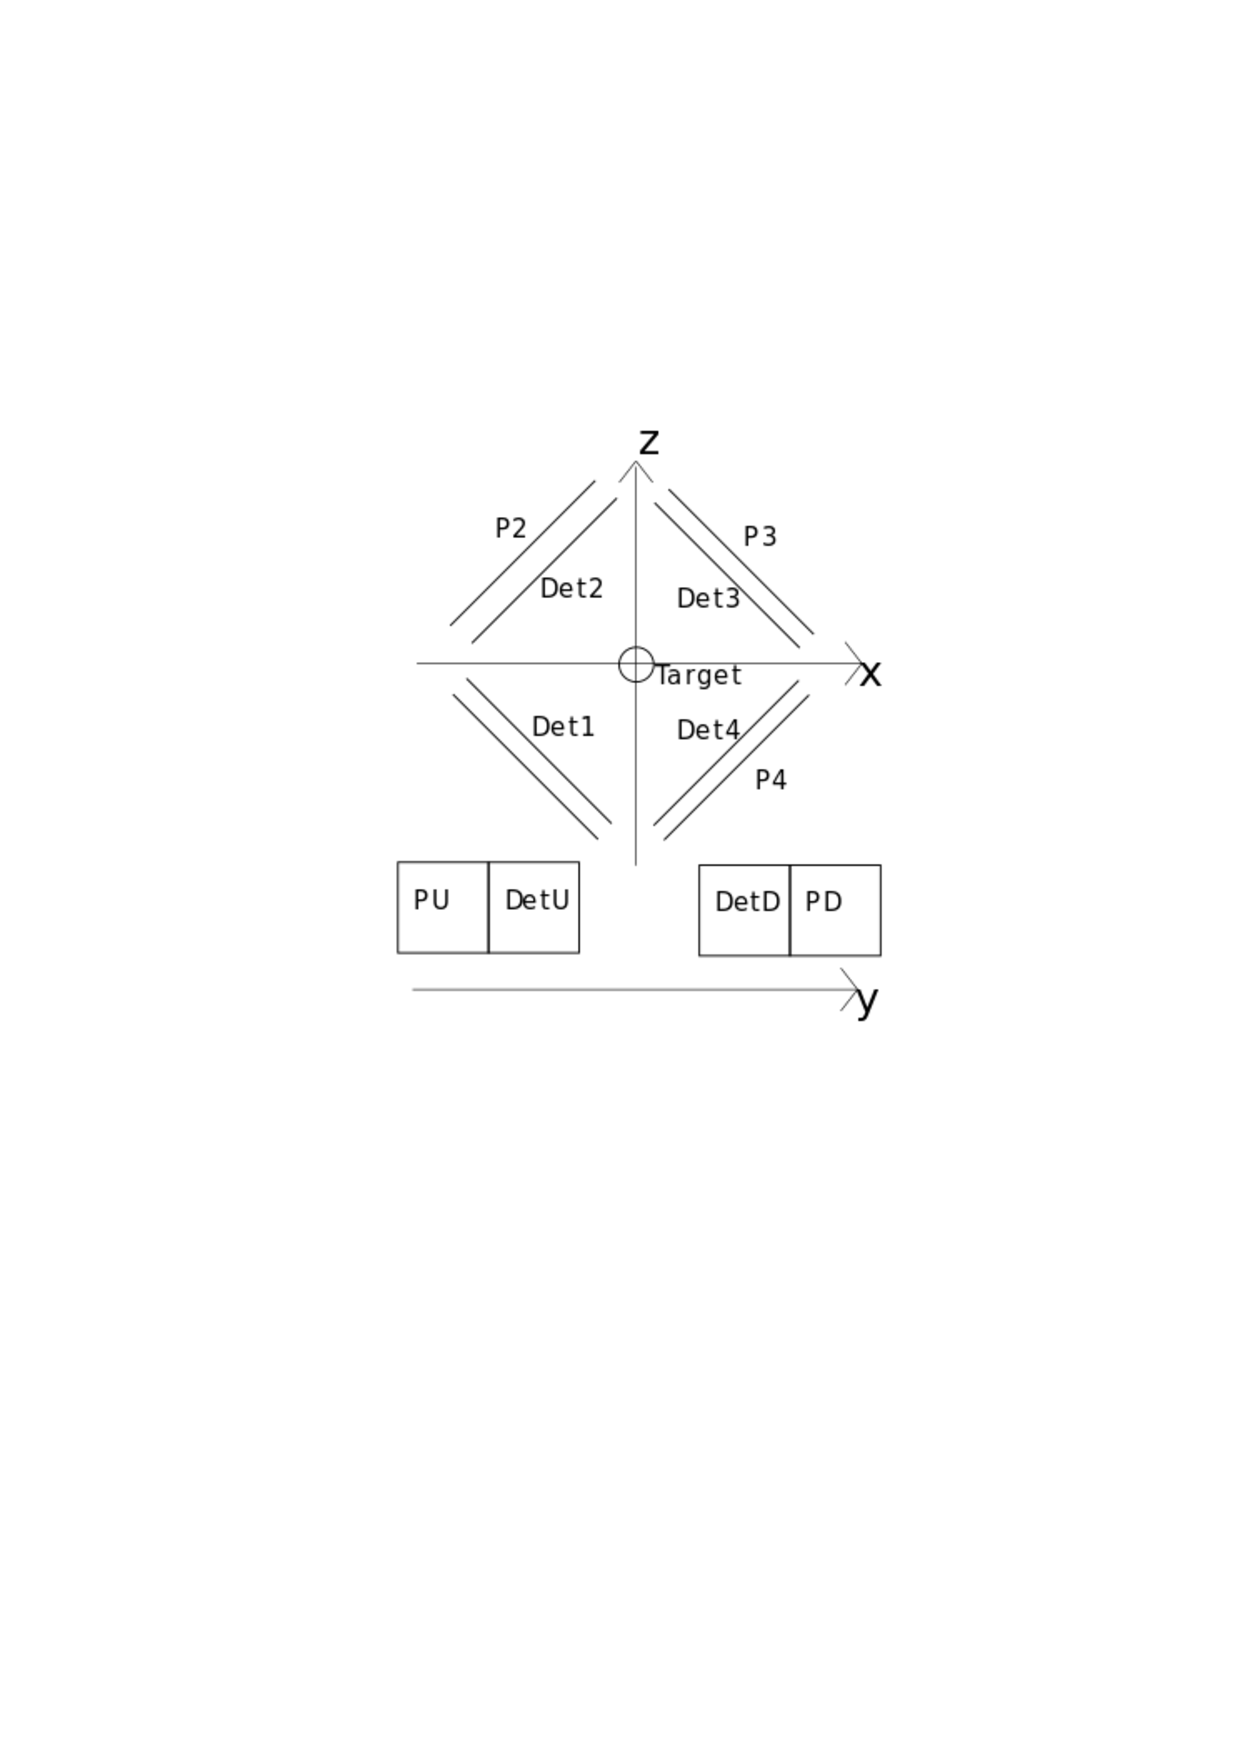
\includegraphics[width=\columnwidth]{../figures/opstilling_better.pdf}
		\end{figure}
		
		\column{0.6\textwidth}
		\small
		\begin{table}
			\begin{tabular}{ll|ll}
				Detektor & Tykkelse {[}$\mu$m{]}  & PAD & Tykkelse{[}$\mu$m{]} 	\\ \hline
				Det1     & 67                     & n/a & n/a                   \\
				Det2     & 1002                   & P2  & 1036                  \\
				Det3     & 65                     & P3  & 1497                  \\
				Det4     & 60                     & P4  & 1490                  \\
				DetU     & 60                     & PU  & 1498                  \\
				DetD     & 1043                   & PD  & 1038                 
			\end{tabular}
		\end{table}		
	\end{columns}


\end{frame}

\begin{frame}{Eksperimentel opsætning}
	\begin{columns}
		\column{0.49\textwidth}
		\begin{figure}
			\centering
			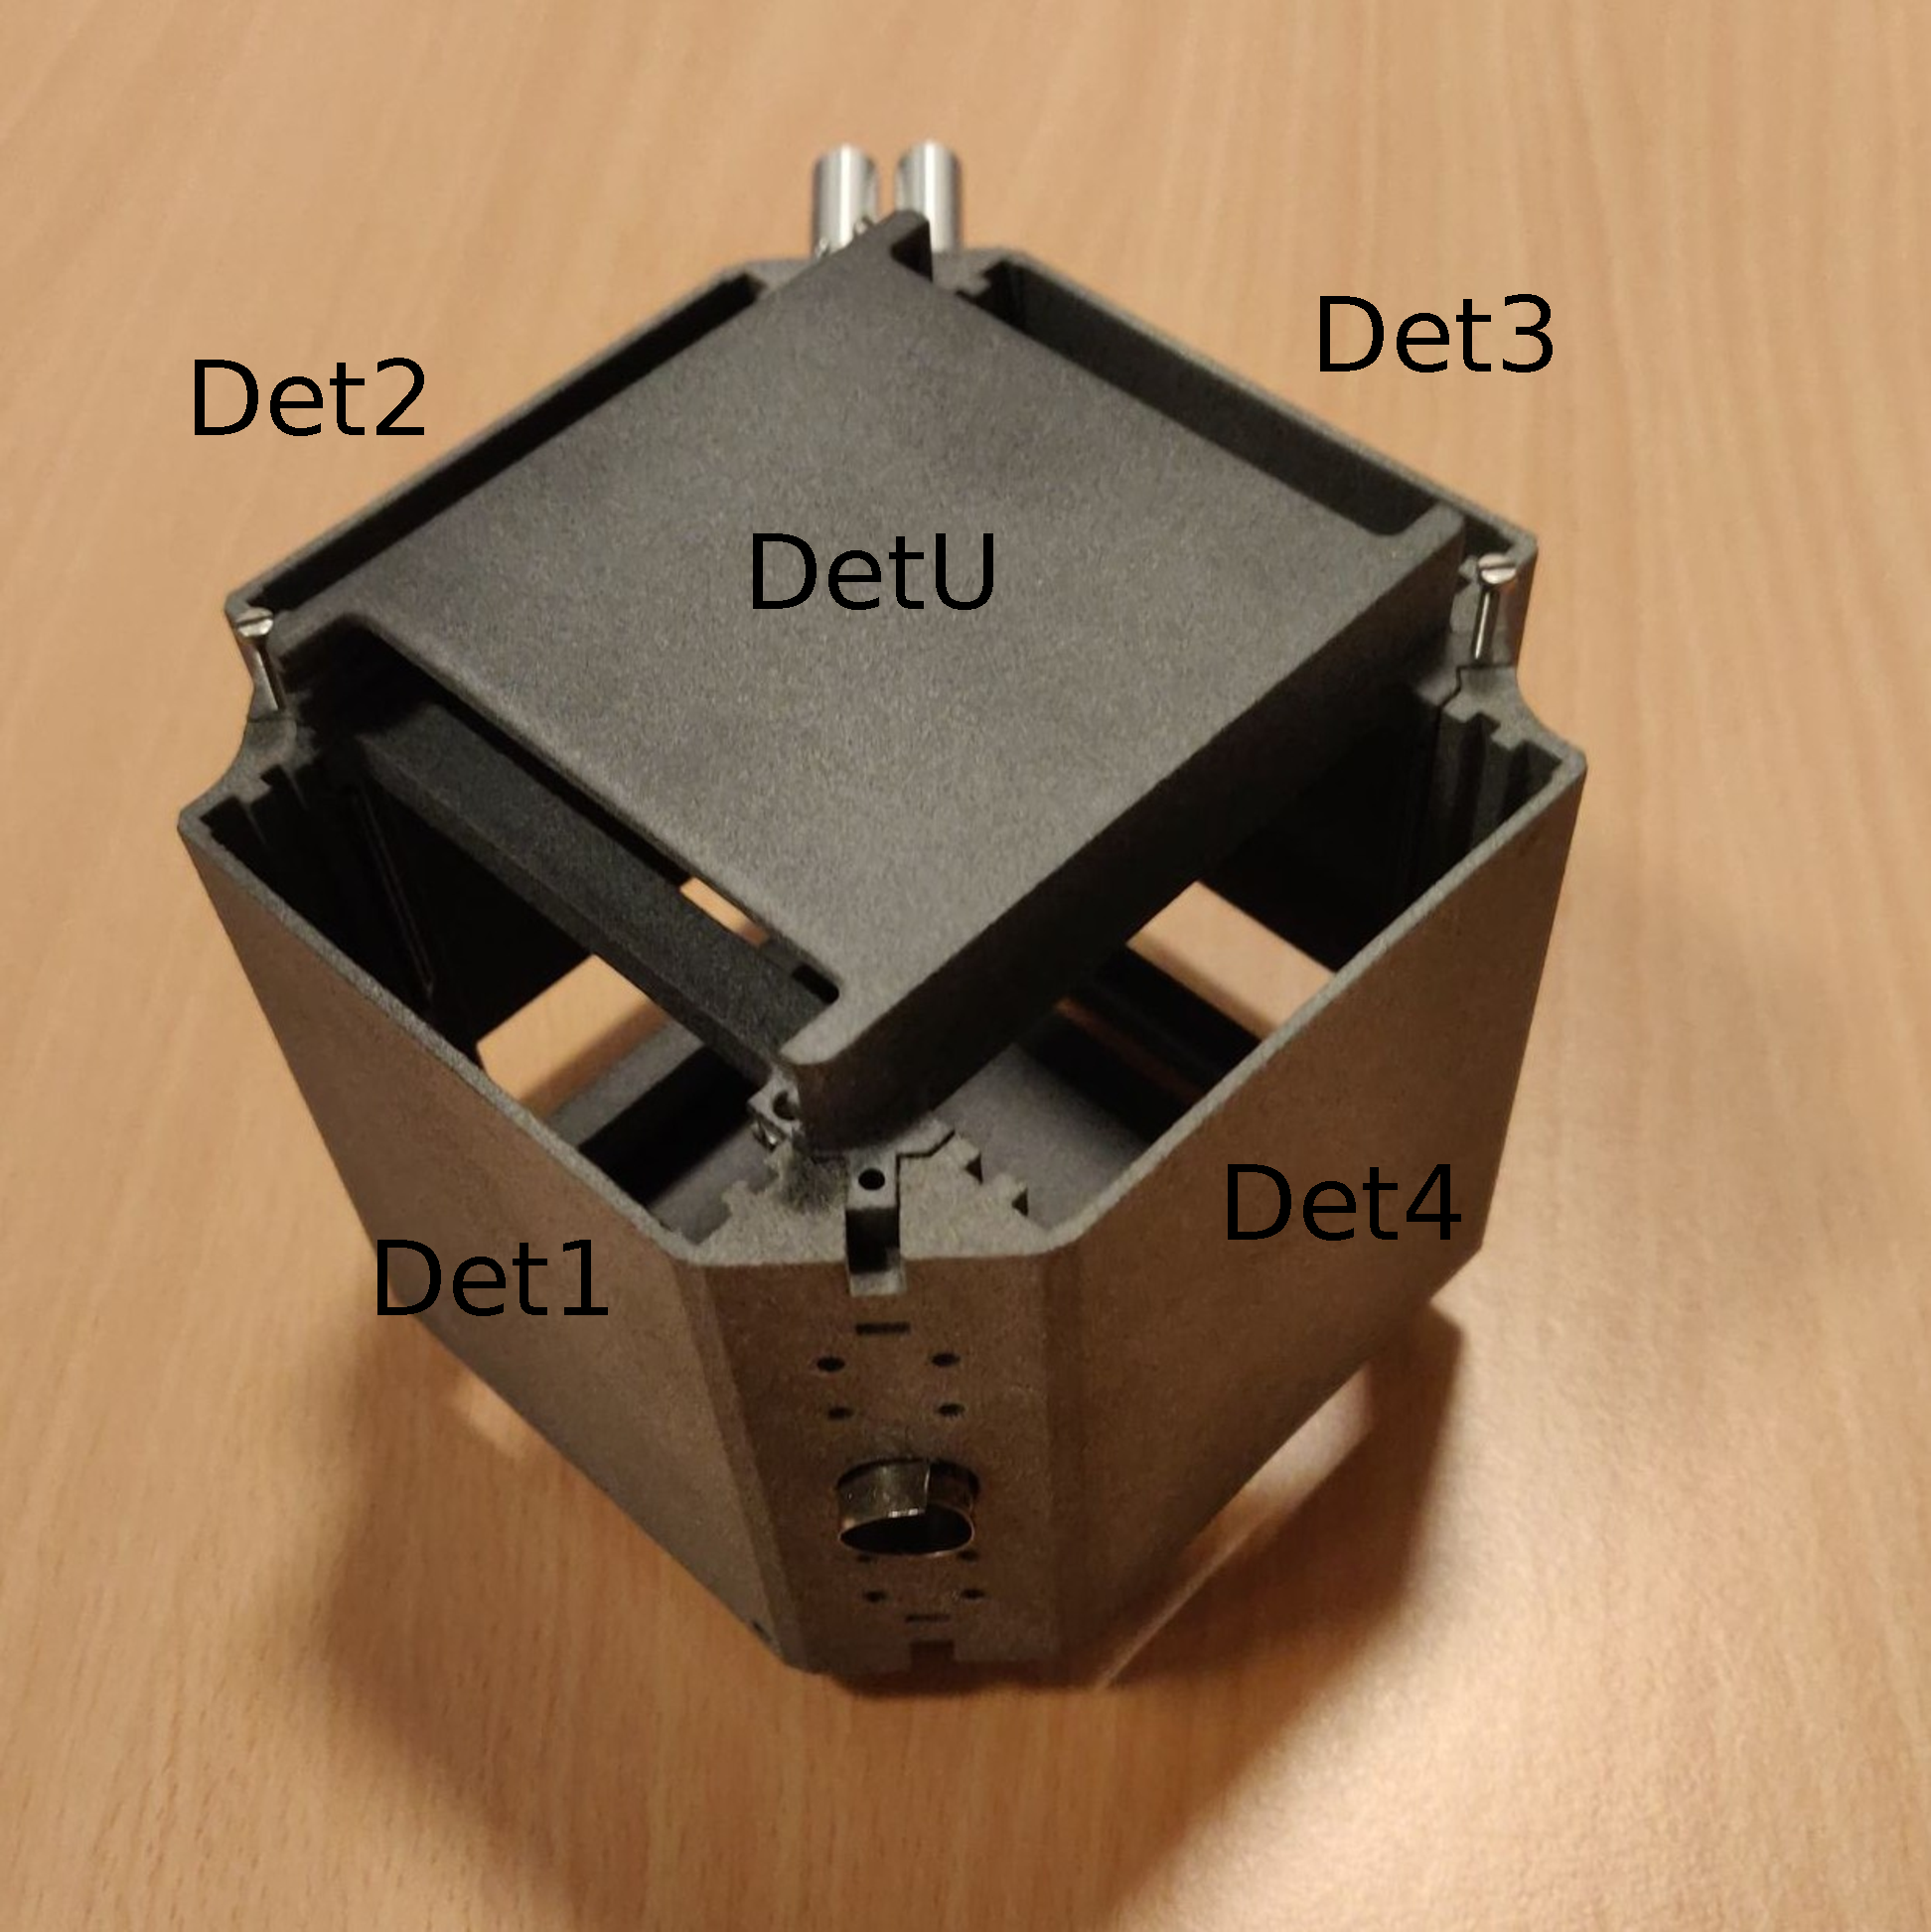
\includegraphics[width=\columnwidth]{../figures/cubepic.pdf}
		\end{figure}
		\column{0.49\textwidth}
		\begin{figure}
			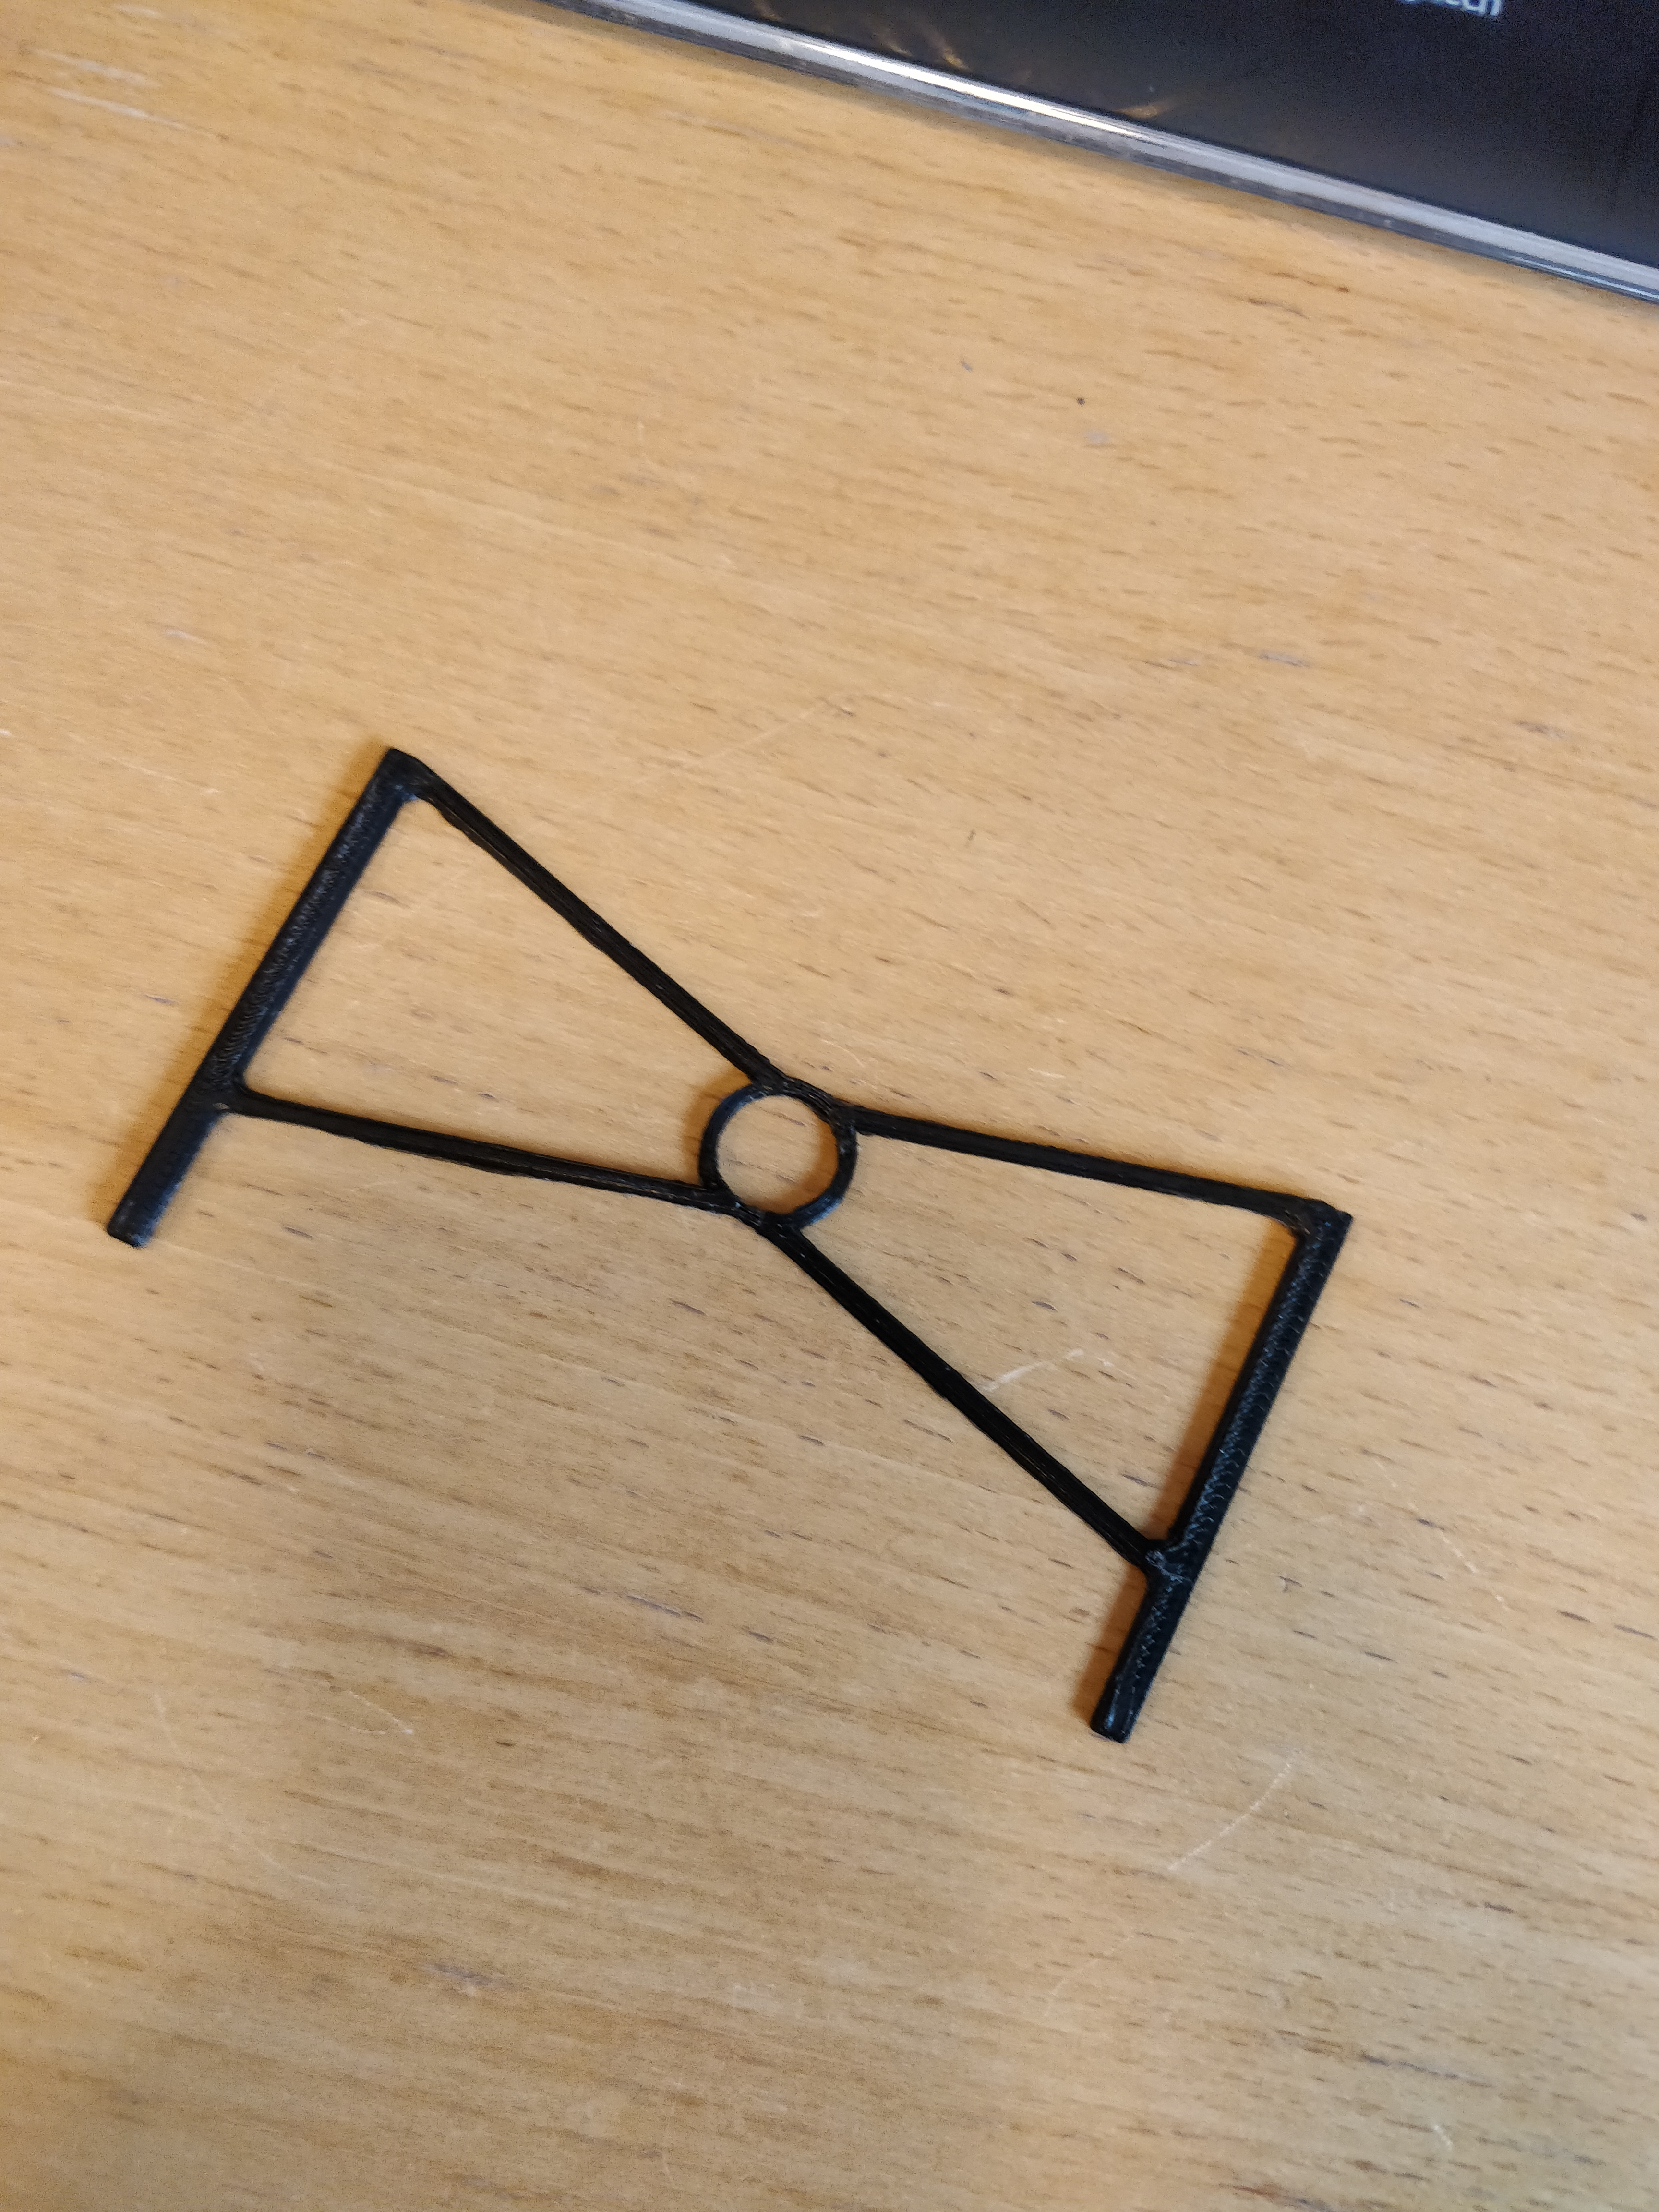
\includegraphics[width=.9\columnwidth]{../figures/targetHolder.jpg}
		\end{figure}
	\end{columns}
\end{frame}

\begin{frame}{Eksperimentel opsætning}
	\begin{columns}
		\column{0.4\textwidth}
		\begin{figure}
			\centering
			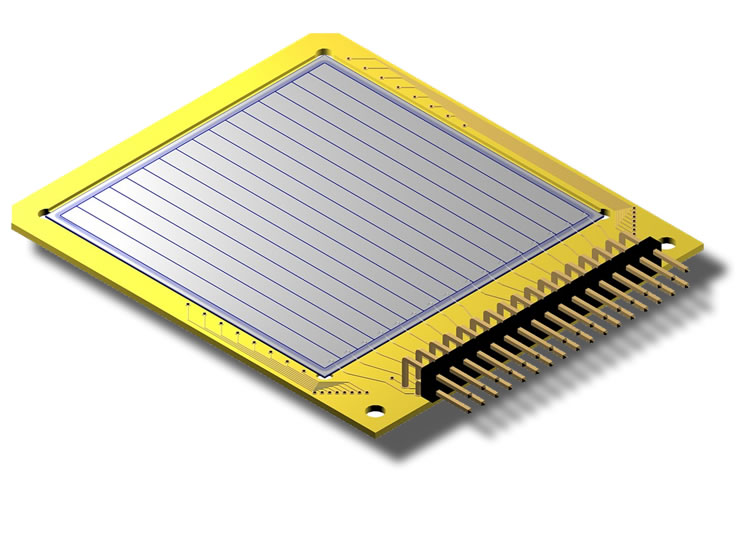
\includegraphics[width=\columnwidth]{../figures/W1.jpg}
		\end{figure}
		$16\times16$ strips\\
		256 pixels 
		\column{0.6\textwidth}
		\begin{figure}
			\centering
			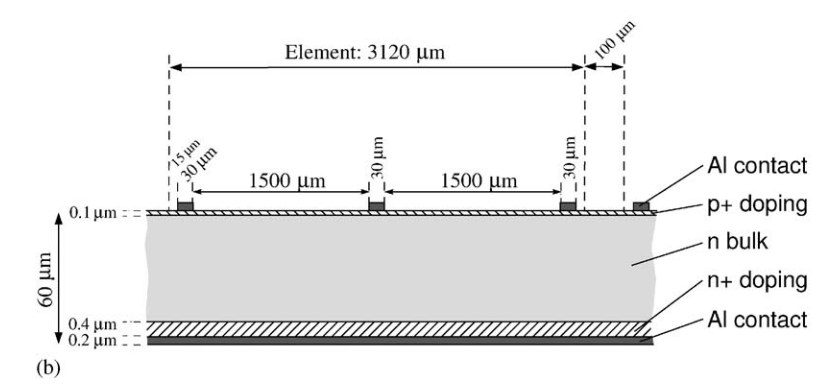
\includegraphics[width=\columnwidth]{../figures/dope.png}
		\end{figure}
	\end{columns}
\end{frame}

\begin{frame}{Software}
	\begin{columns}
		\column[]{0.6\textwidth}
	\begin{itemize}
		\onslide<2->{\item ROOT}
		\begin{itemize}
			\onslide<3->{\item C++ framework}
		\end{itemize}
		\onslide<4->{\item AUSA}
		\begin{itemize}
			\onslide<5->{\item Unpacker: Rå data til ROOT \texttt{Tree}}
			\onslide<6->{\item Calibrator: Detektor kalibrering}
			\onslide<7->{\item Sorter: Konvertere strip signaler til pixel hit}
		\end{itemize}
	\end{itemize}
	\column[]{0.4\textwidth}
	\onslide<7->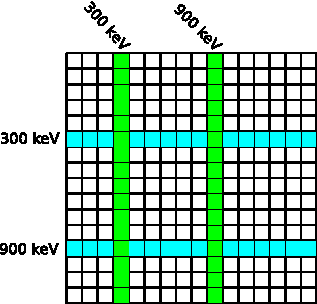
\includegraphics[width=\columnwidth]{../figures/sorter.pdf}
\end{columns}
\end{frame}

\begin{frame}{Kalibrering}
	\begin{columns}
		\column{0.5\textwidth}
		Kendte kilder:\\
		\begin{table}[H]
			\centering
			\begin{tabular}{ll}
				Isotope & $E_\alpha \ [keV]$  \\ \hline
				\isotope[148][]{Gd}		& 3182.690         \\
				\isotope[239][]{Pu}		& 5105.5           \\
				& 5144.3           \\
				& 5156.59          \\
				\isotope[244][]{Cm}		& 5762.64          \\
				& 5804.96          \\ 
			\end{tabular}
		\end{table}
	
		\column{0.5\textwidth}
		\begin{figure}
			\centering
			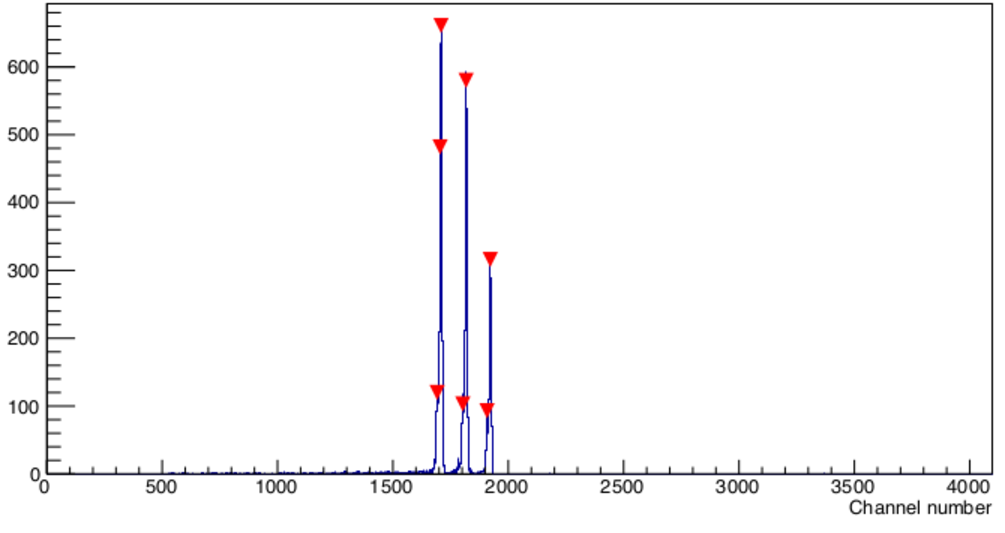
\includegraphics[width=\columnwidth]{../figures/cali/det1f1-cropped-Mia.pdf}
		\end{figure}
		\begin{figure}
			\centering
			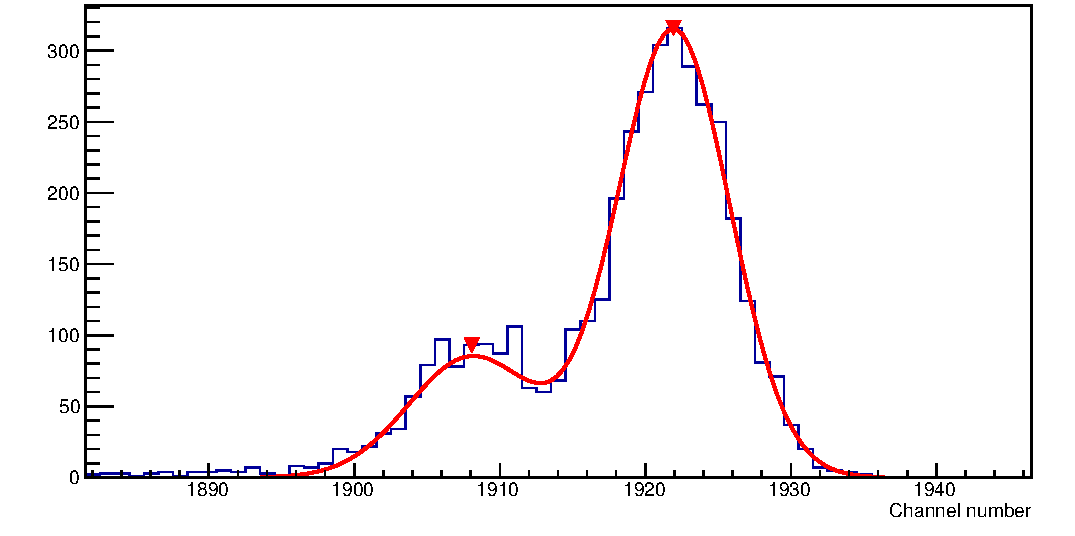
\includegraphics[width=\columnwidth]{../figures/cali/det1f1PeakMostLeft-cropped.pdf}
		\end{figure}
	\end{columns}
\end{frame}


\section{Data reduktion}

\begin{frame}{Identificer partikler}
	Forskellige energi afsætning\\
	\al-partikler bliver stoppet af \SI{60}{\mu m}\\
	\be-partikler afsætter \SI{300}{keV} - \SI{500}{keV} pr. mm silicium\\
	Overlappende energi\\
	\be-partikler bliver opfanget af PAD
\end{frame}

\begin{frame}{Identificer partikler}
	
\end{frame}
%\section{Effektivitet af cuts}
\begin{frame}{Effekten af cuts}
	Hvordan ser usorteret data ud?\\
	\begin{figure}
		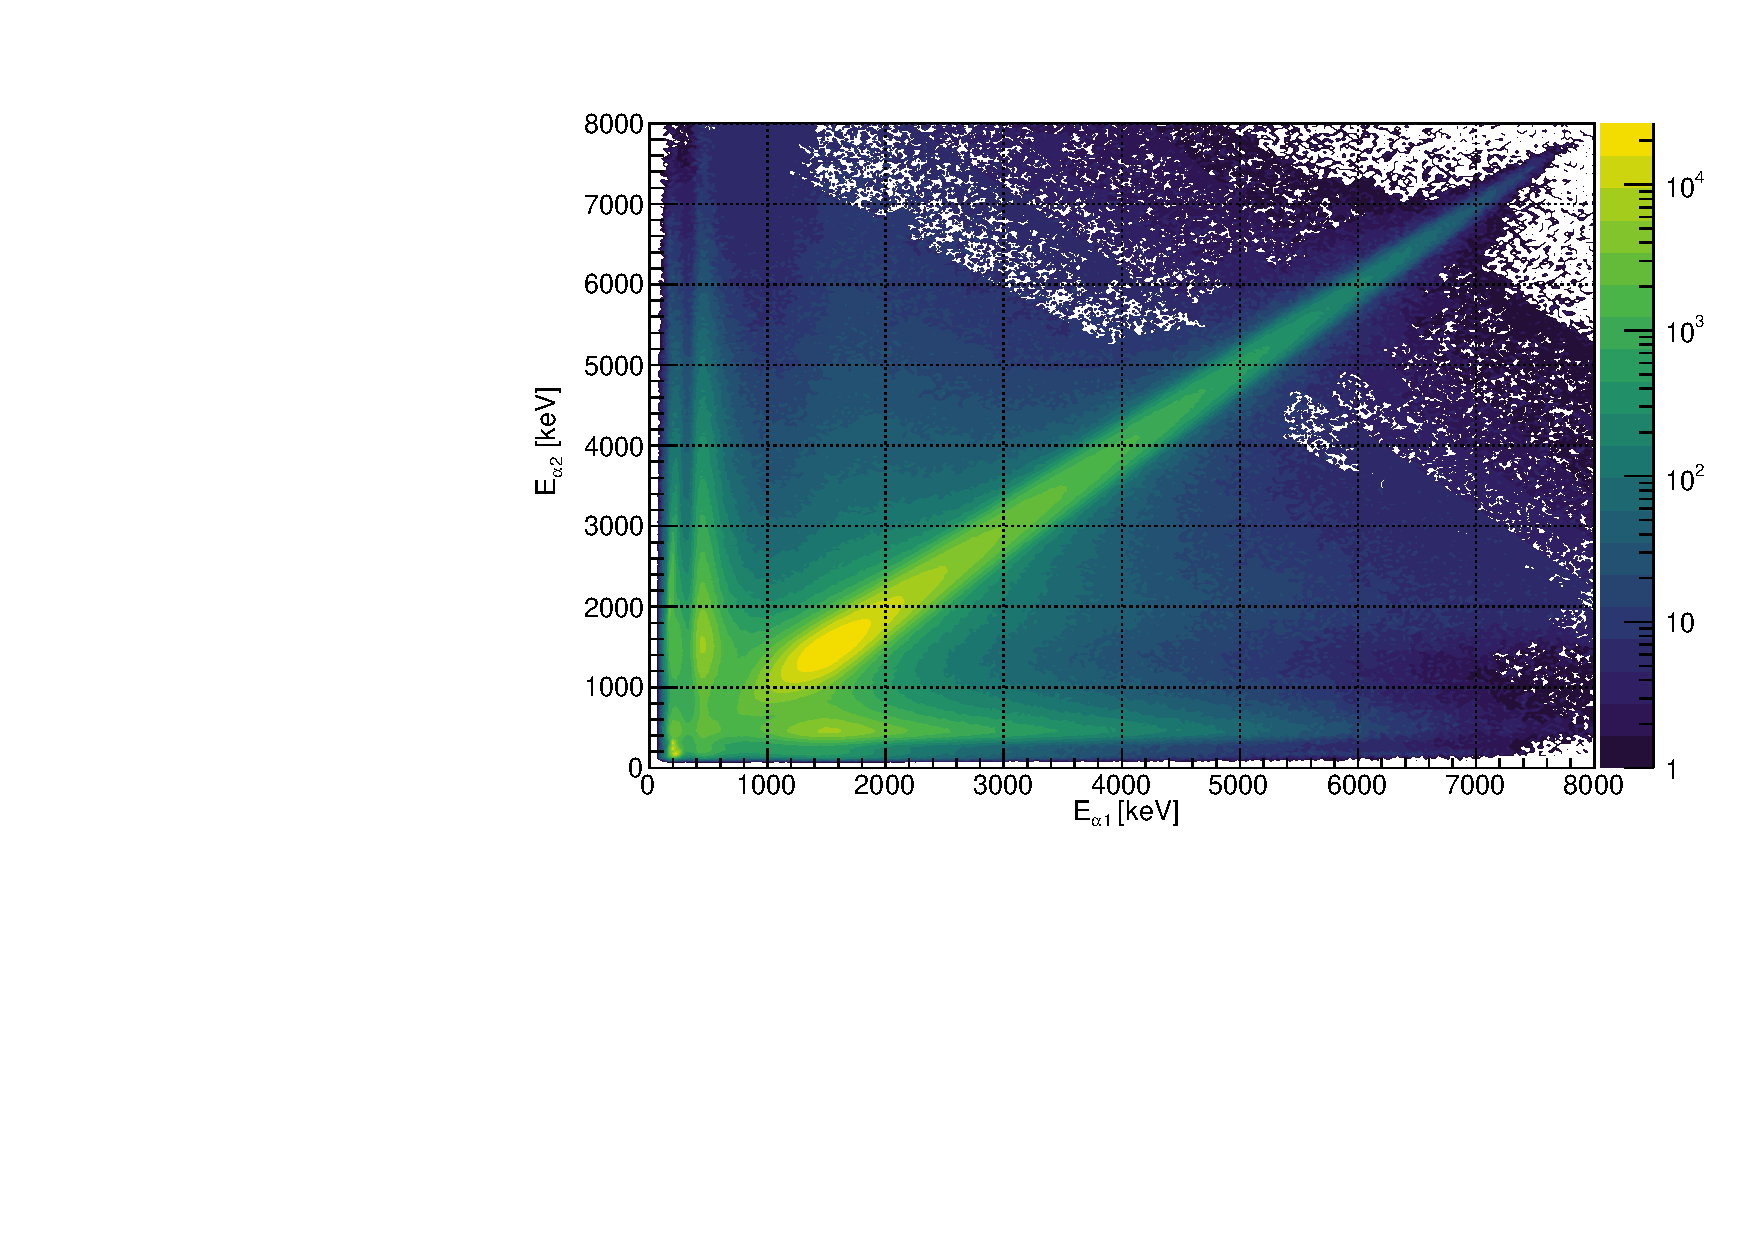
\includegraphics[width=0.7\columnwidth]{../figures/EENoCuts.pdf}
	\end{figure}
\end{frame}

\begin{frame}{Effekten af vinkel cut}
	Indbyrdes vinkel på maksimalt $161\degree$\\
	\begin{figure}
		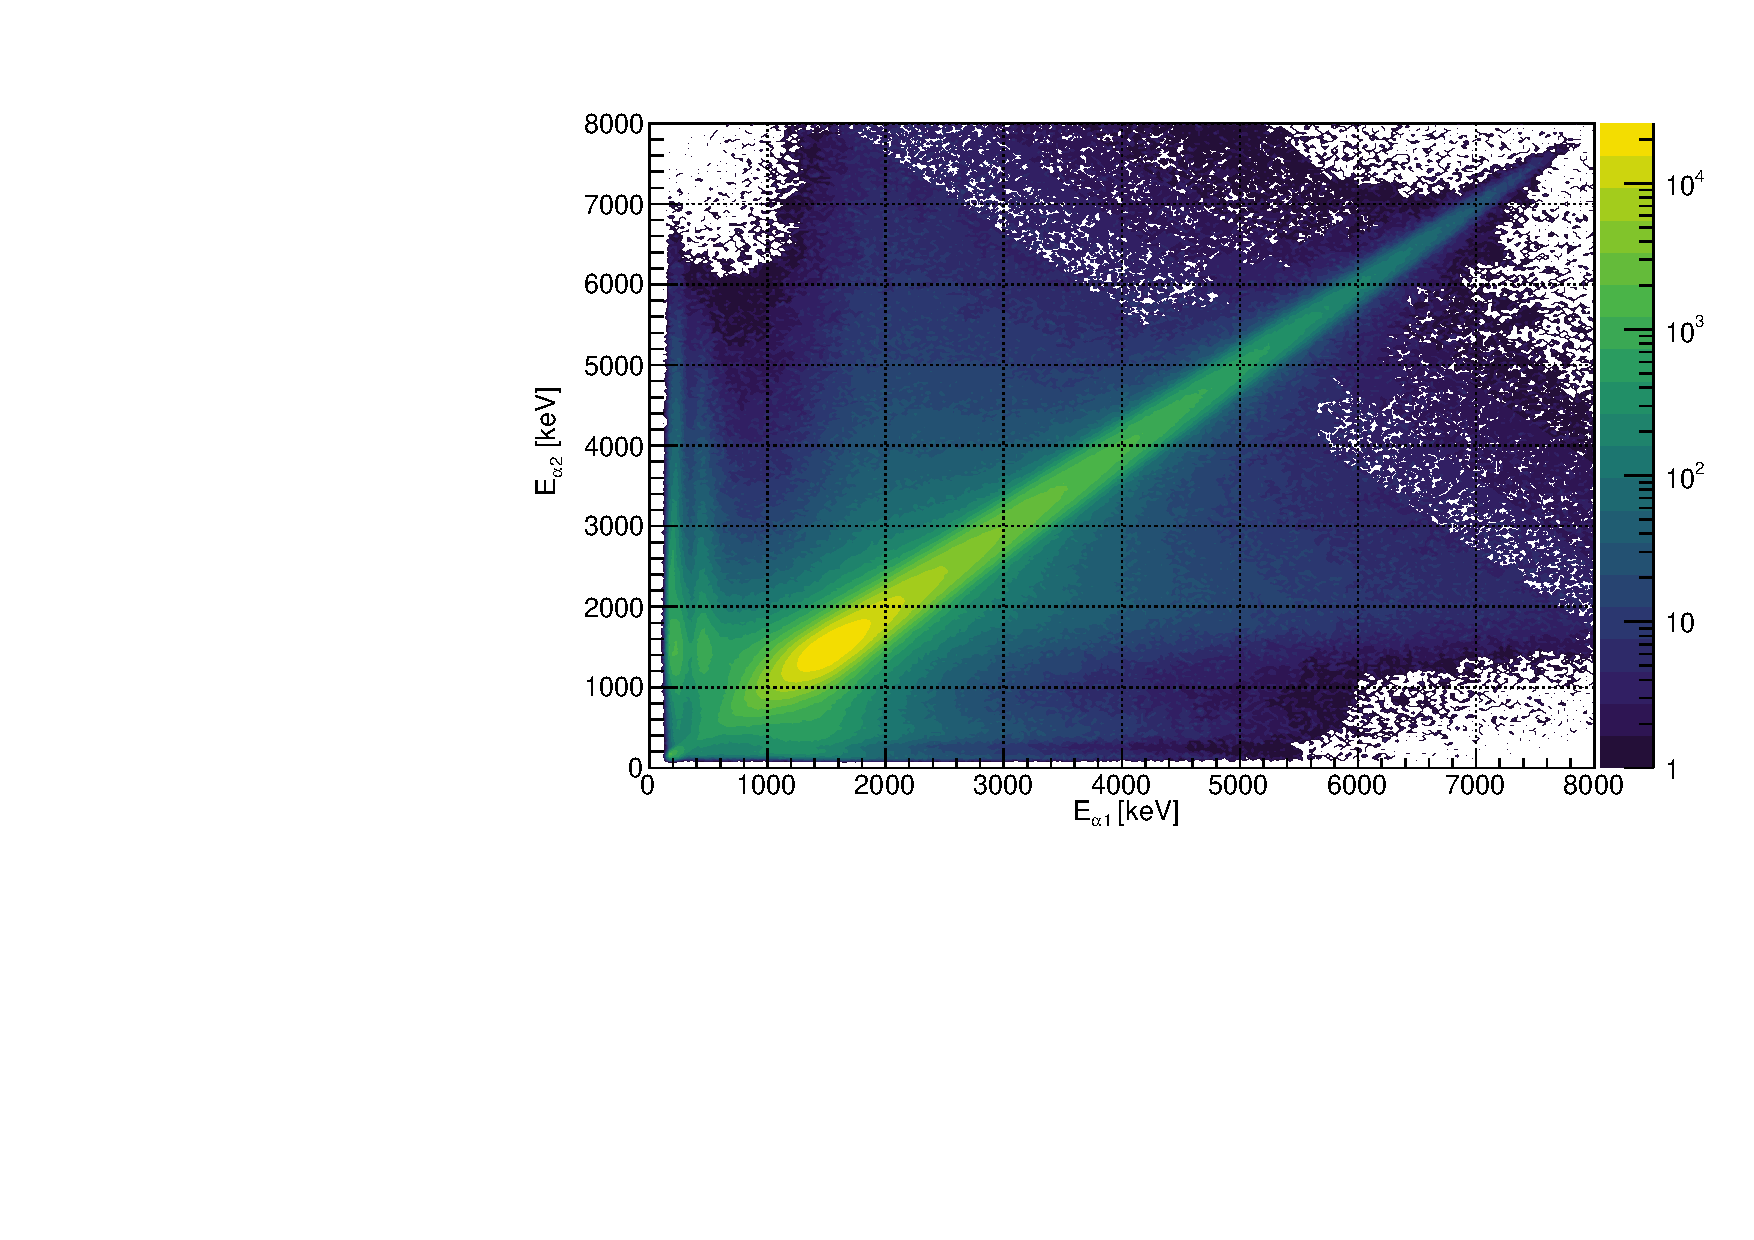
\includegraphics[width=0.7\columnwidth]{../figures/EEAngleCut.pdf}
	\end{figure}
\end{frame}

\begin{frame}{Effekten af impuls cut}
	Total impuls på maksimalt \SI{40}{MeV/c}
	\begin{figure}
		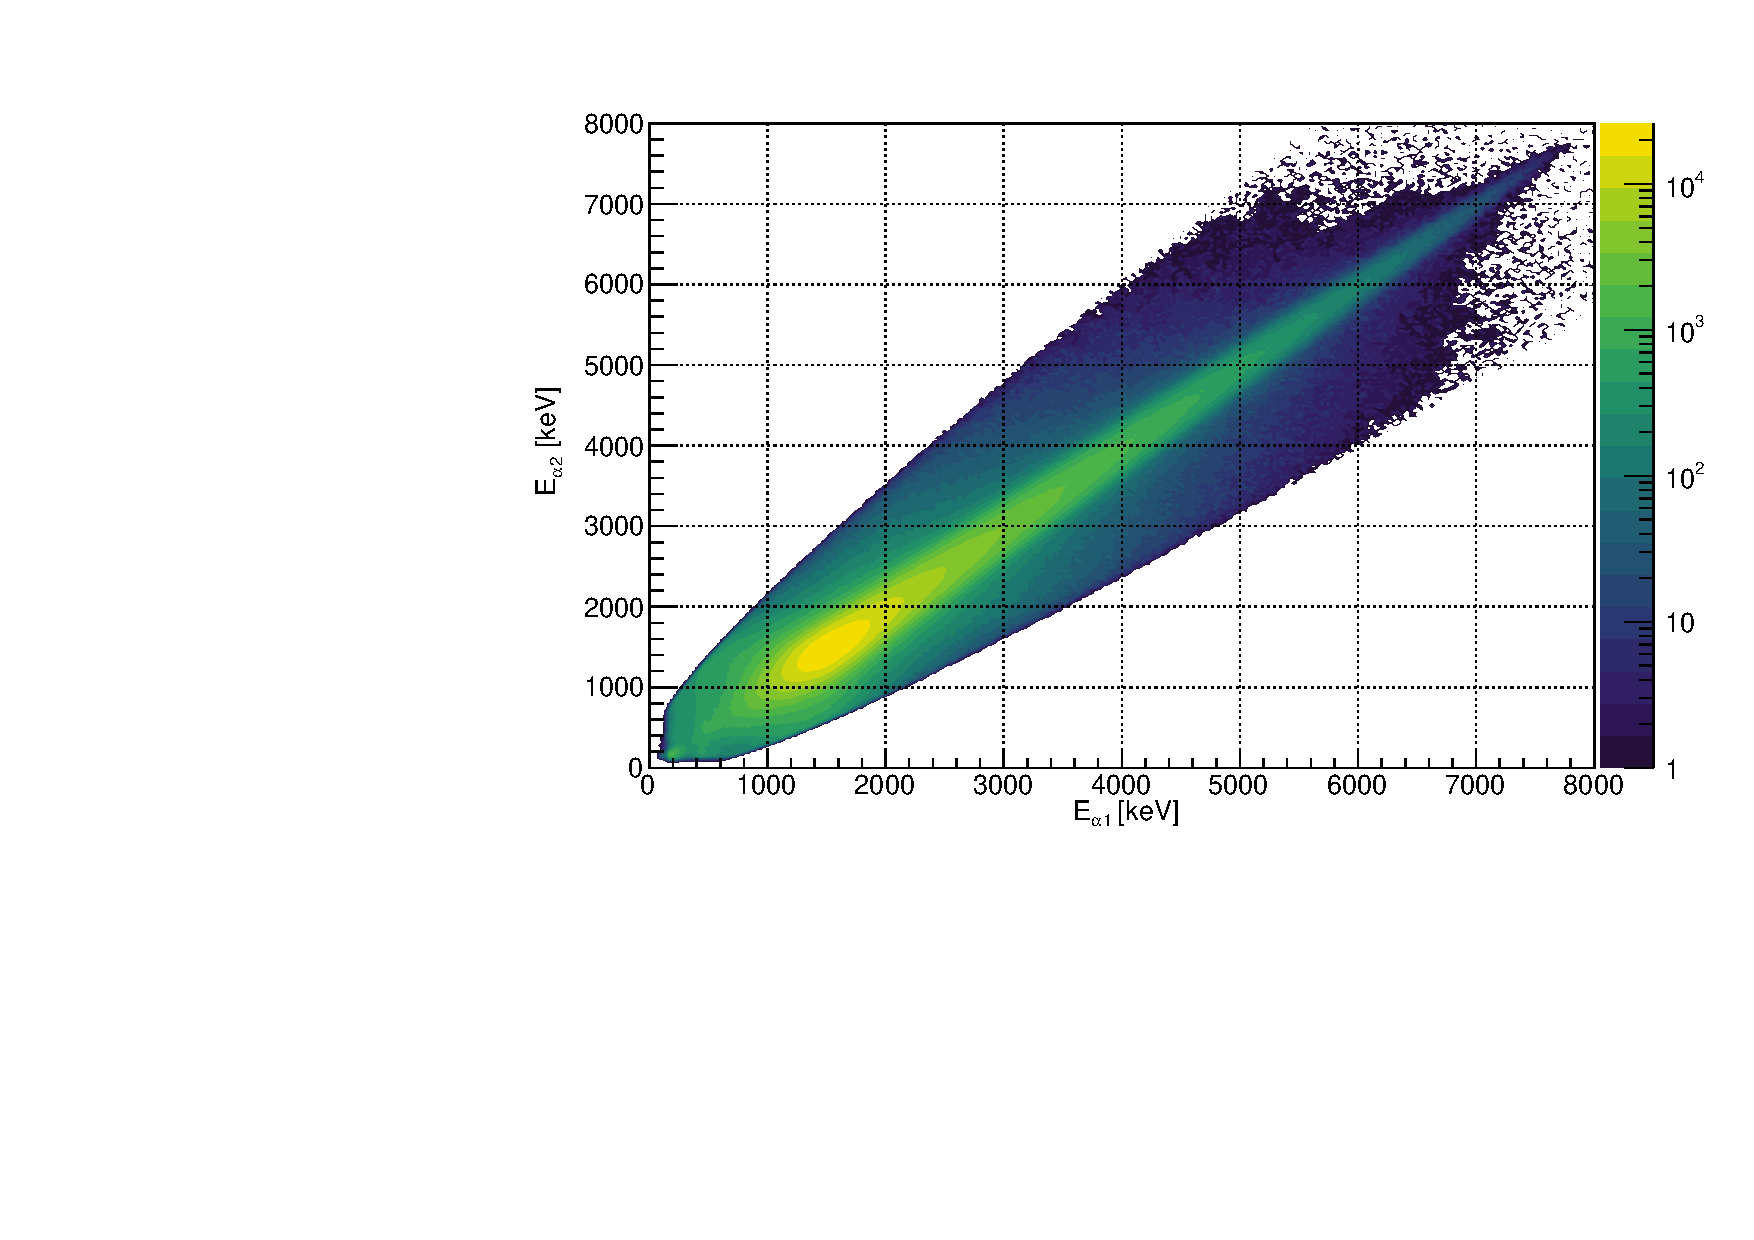
\includegraphics[width=.7\columnwidth]{../figures/EEMomentumCut.pdf}
	\end{figure}
\end{frame}

\begin{frame}{Effekten af \be-multiplicitet cut}
	Minimum 1 \be-partikel i et event
	\begin{figure}
		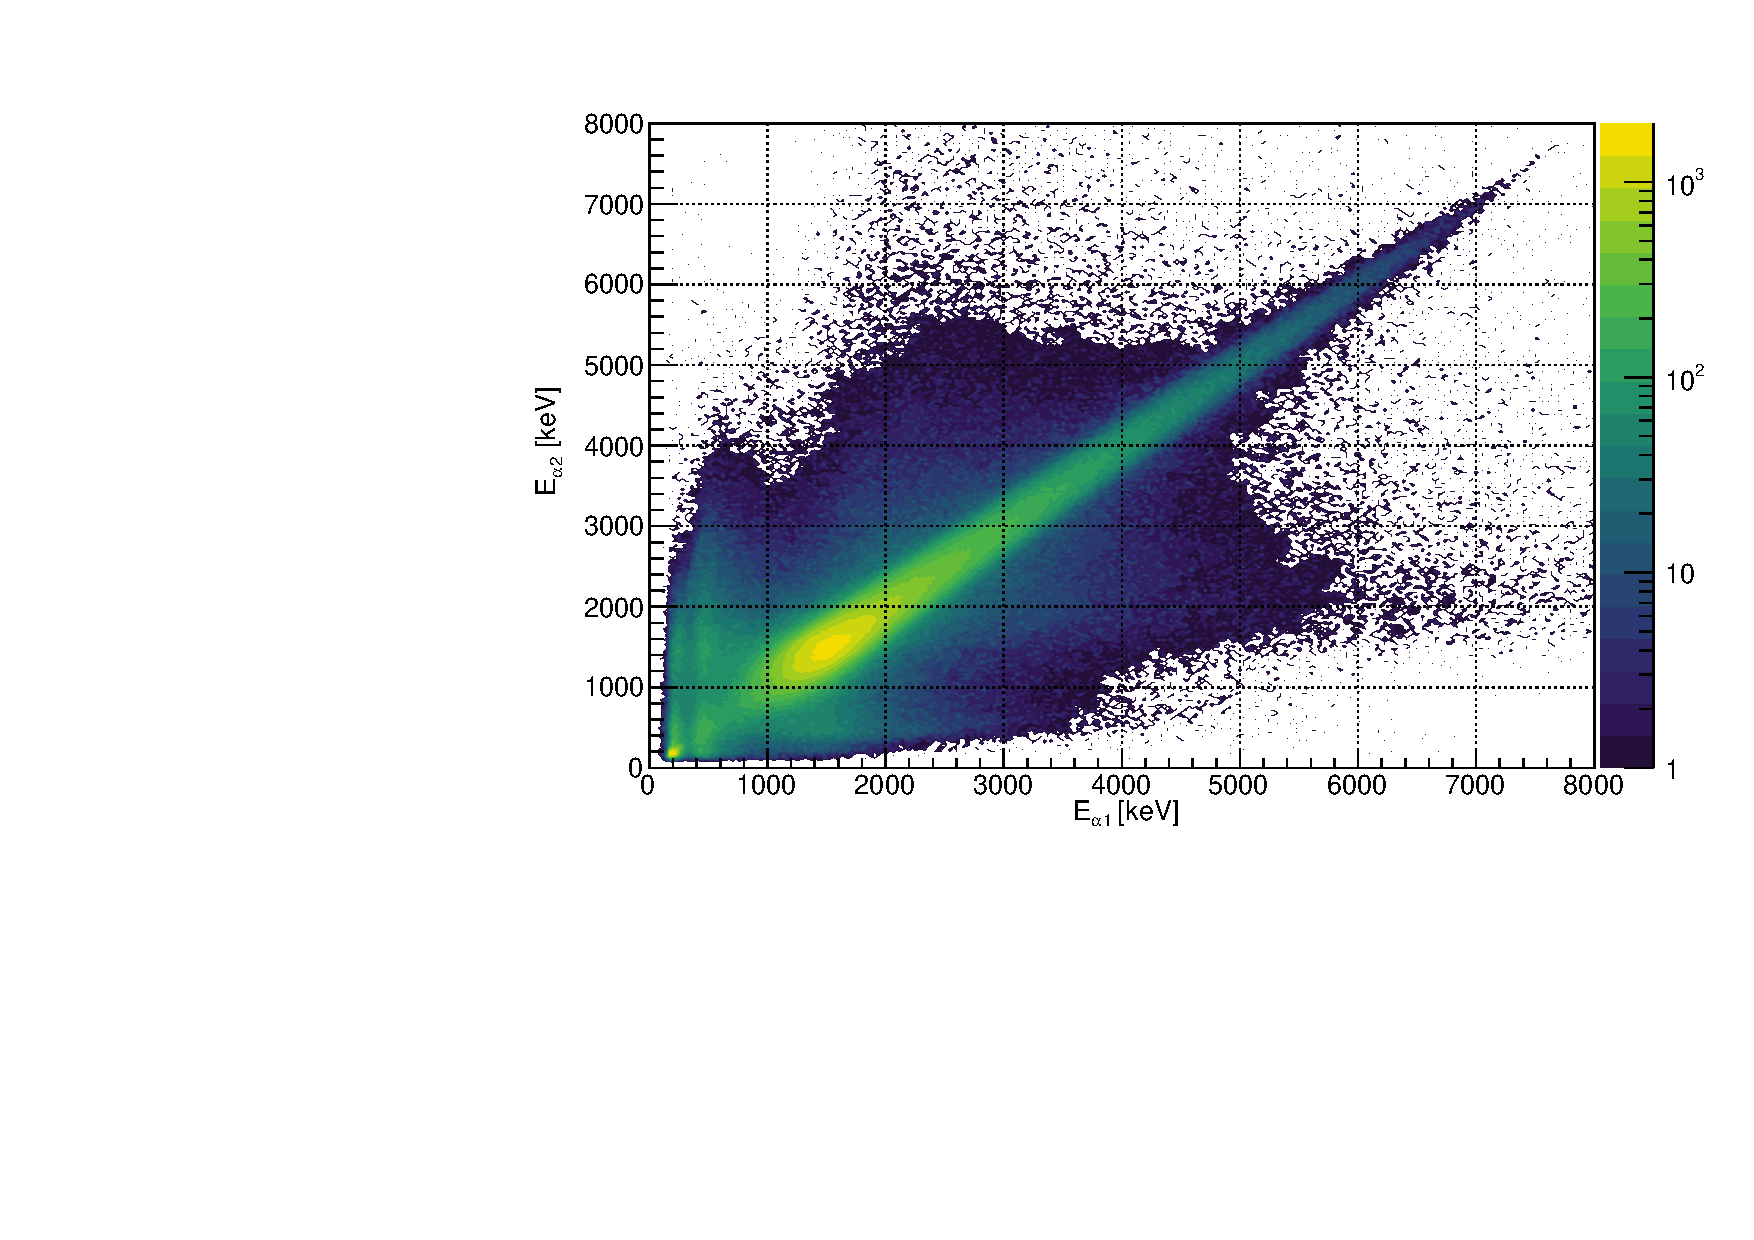
\includegraphics[width=.7\columnwidth]{../figures/EEBetaMulCut.pdf}
	\end{figure}
\end{frame}

\begin{frame}{Effekten af alle cuts}
	Alle cuts 
	\begin{figure}
		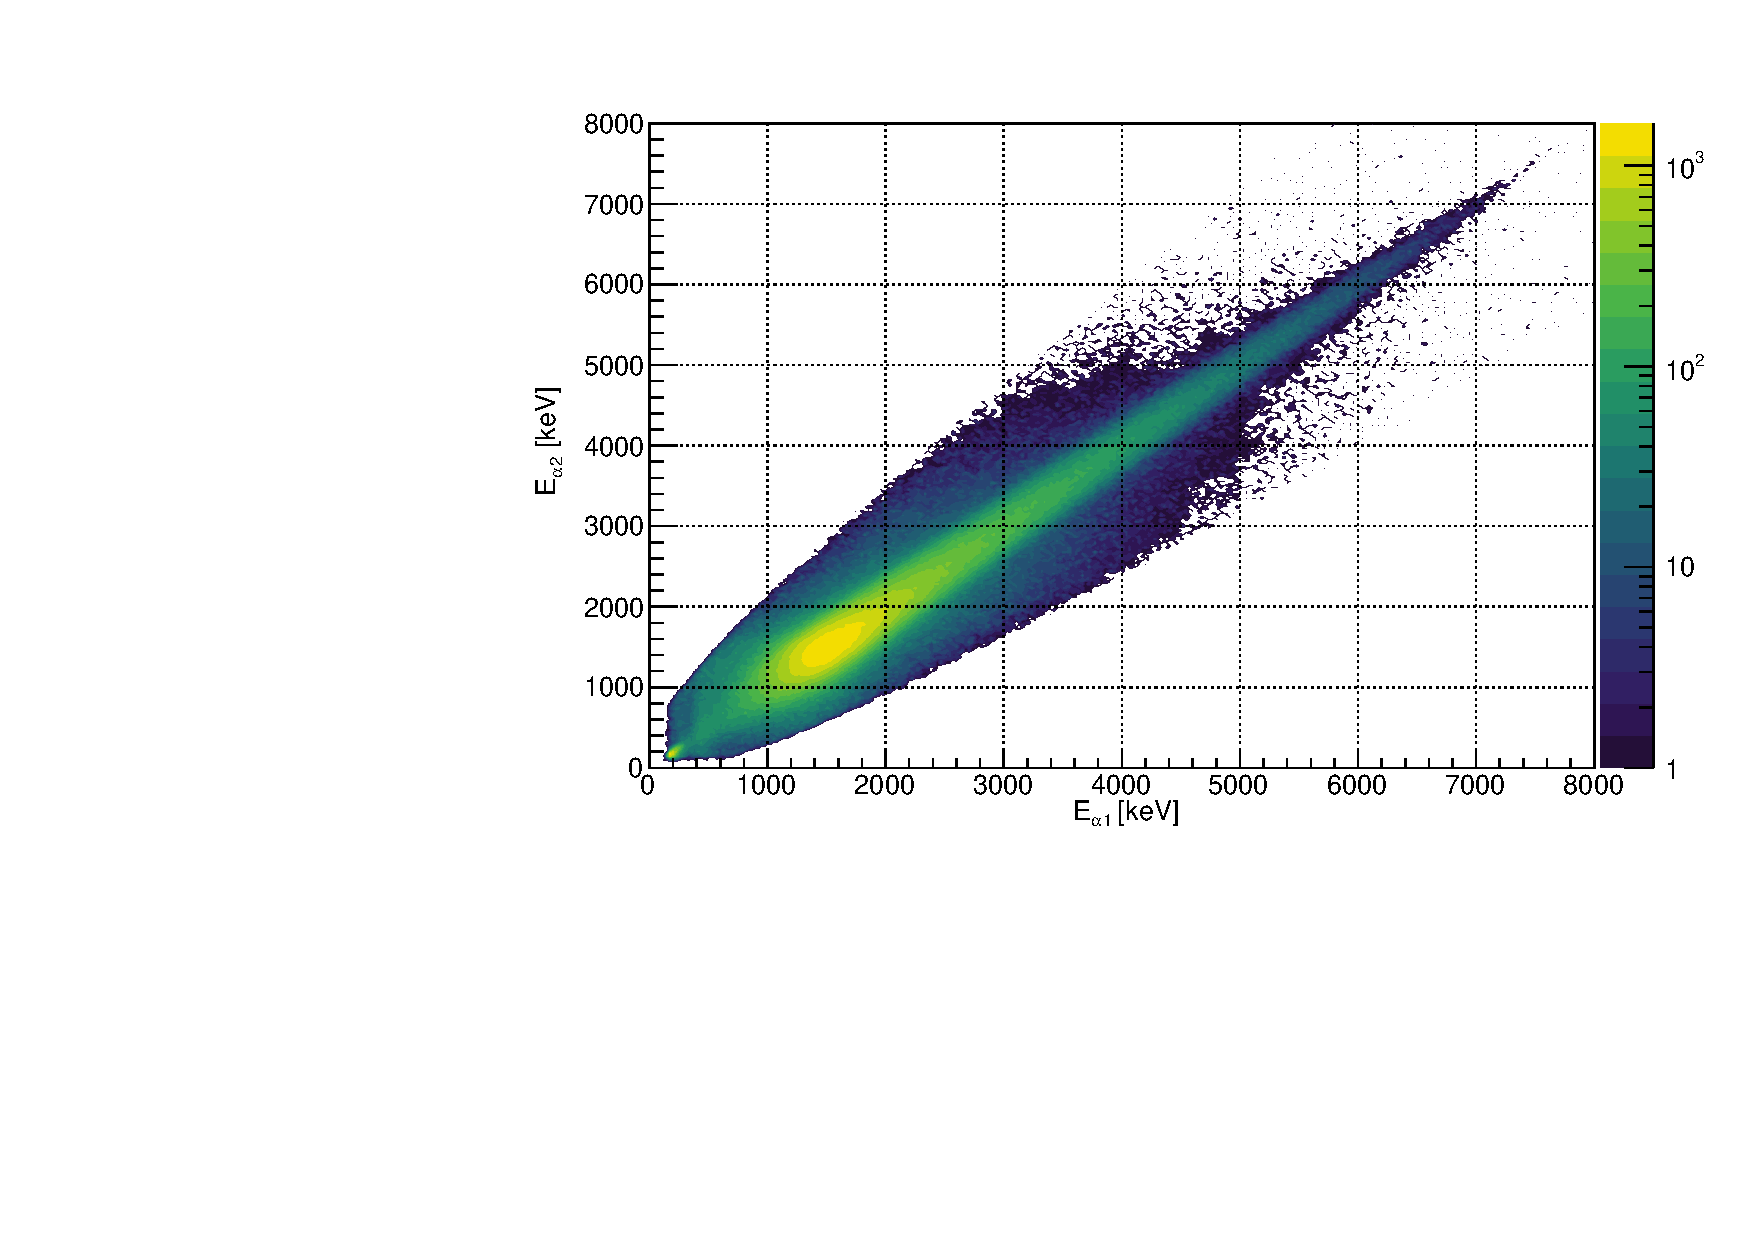
\includegraphics[width=.7\columnwidth]{../figures/EE.pdf}
	\end{figure}
\end{frame}

\begin{frame}{Cut sammenligning}
	Energi spektrum for enkelt \al-partikel
	\begin{figure}
		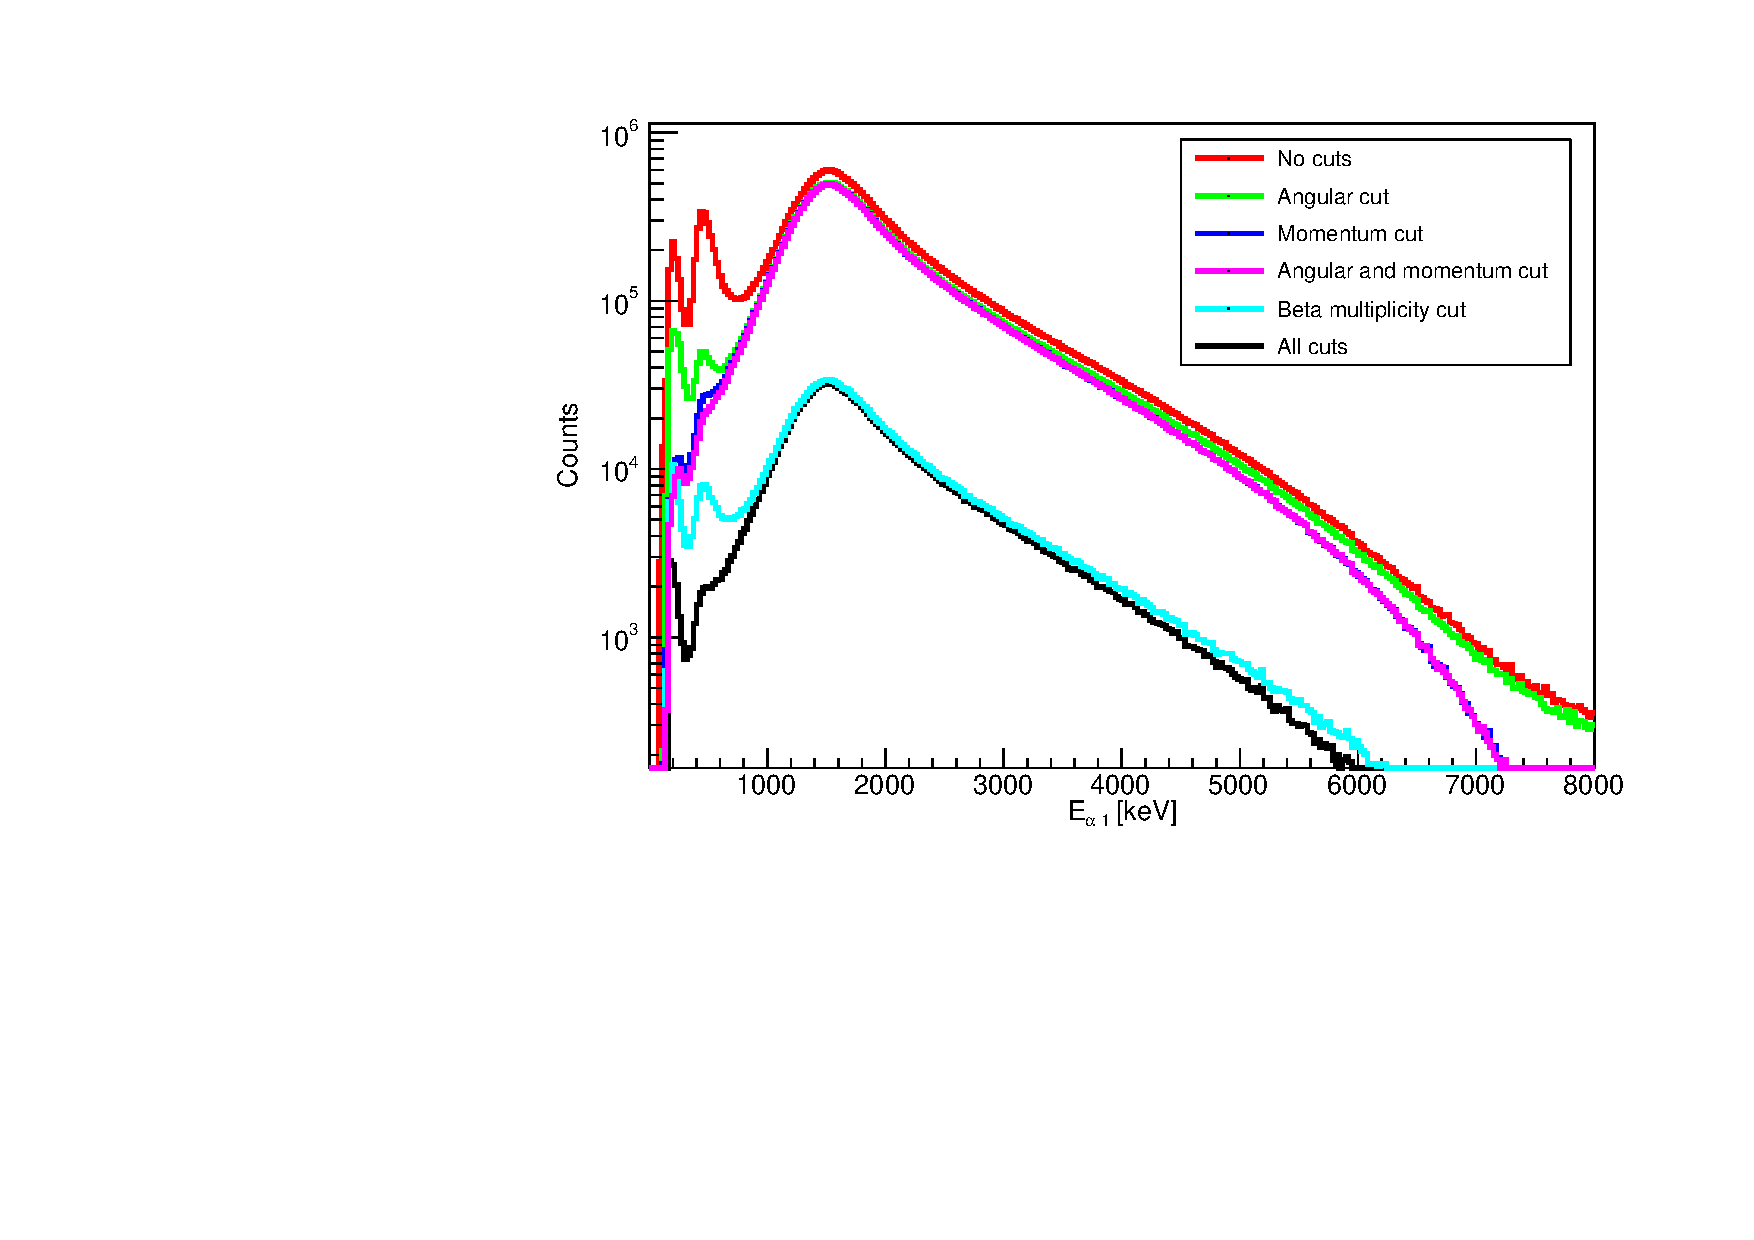
\includegraphics[width=.7\columnwidth]{../figures/cutCompare.pdf}
	\end{figure}
\end{frame}

\begin{frame}{\be\ energi spektrum}
	Falske \be\ identificeringer?
	\begin{figure}
		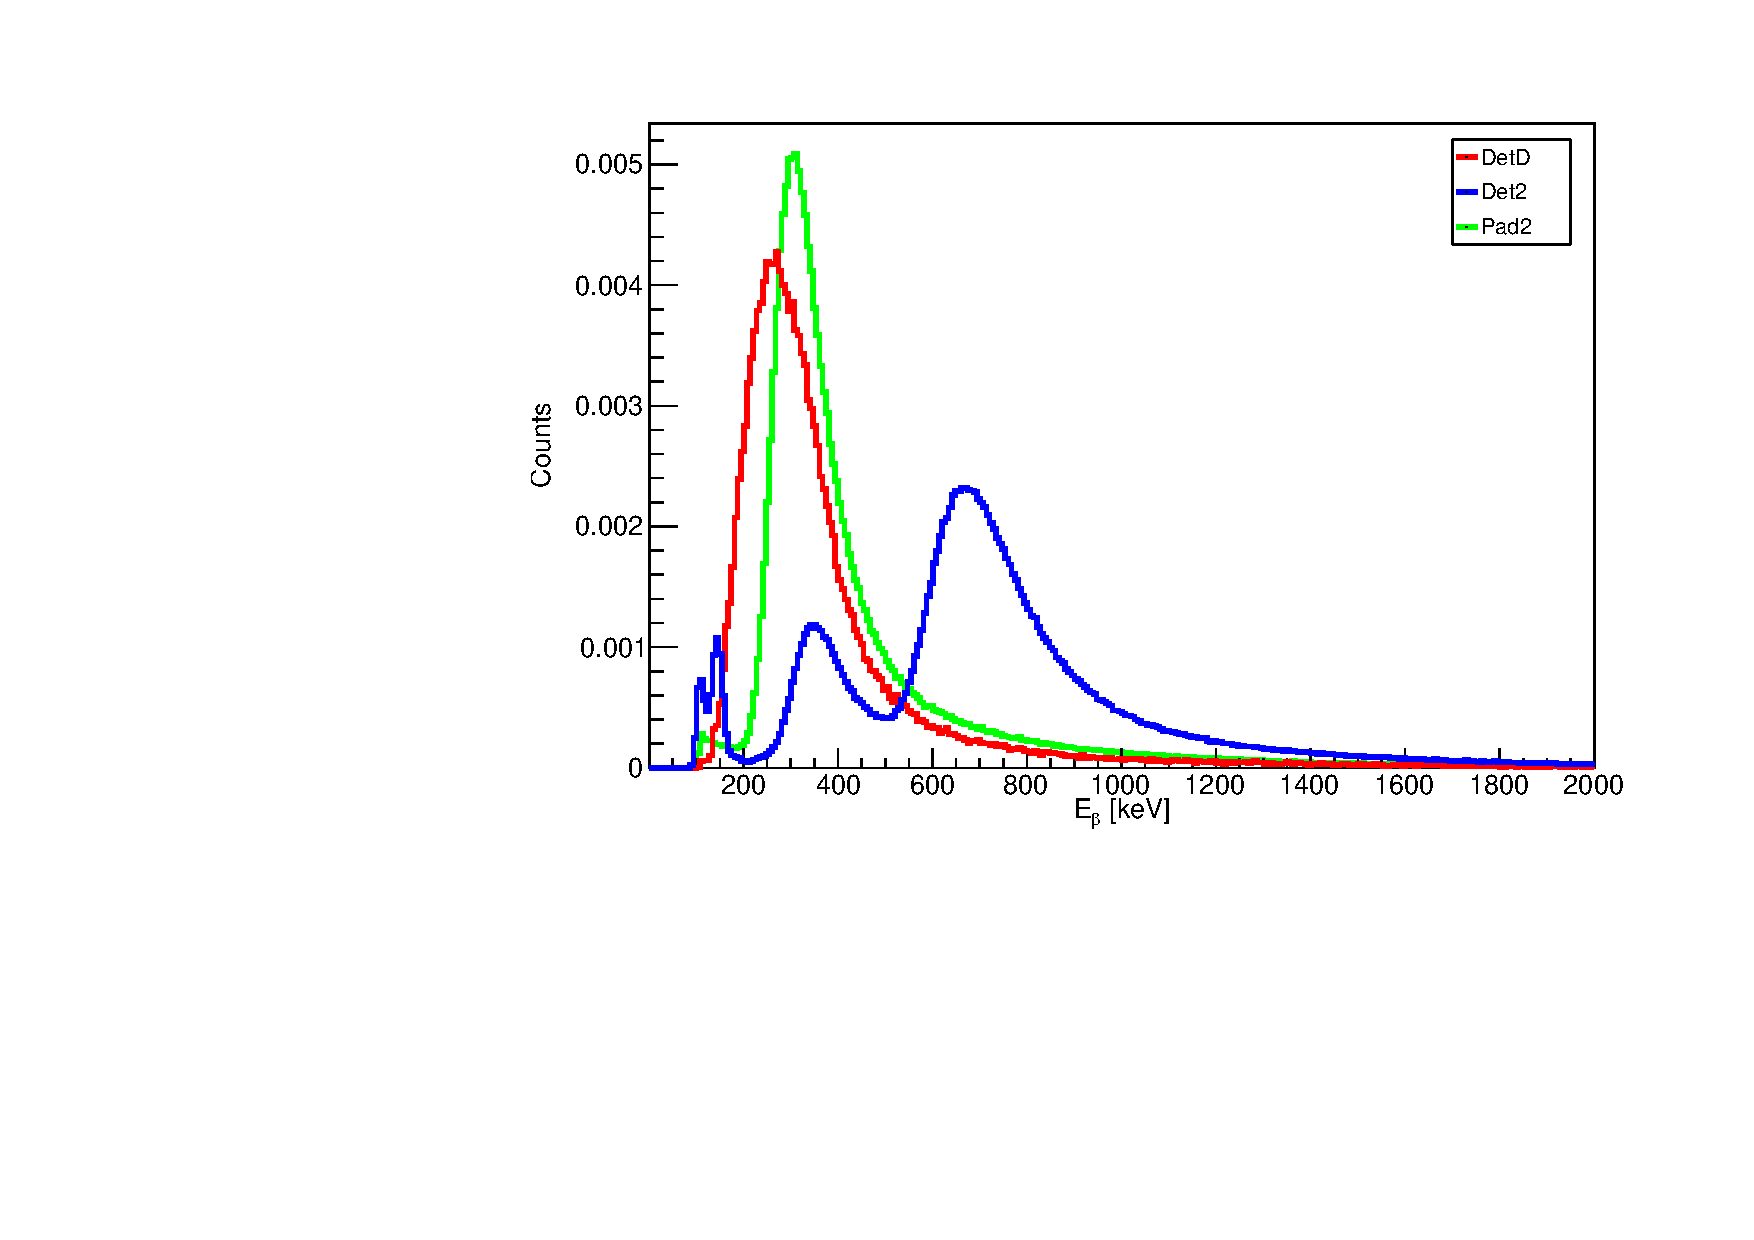
\includegraphics[width=.7\columnwidth]{../figures/betaSpec.pdf}
	\end{figure}
\end{frame}

\section{Data analyse}

\begin{frame}{Excitations spektrum for $^8$Be}
	\begin{itemize}
		\onslide<2->{\item Energi for summen af to \al-partikler}
		\onslide<3->{\item Sammenligning med tidligere målinger }
		\onslide<4->{\item God overensstemmelse for peak}
		\onslide<5->{\item Lav energiniveau divagere meget fra hinanden}
	\end{itemize}

	\onslide<2->
	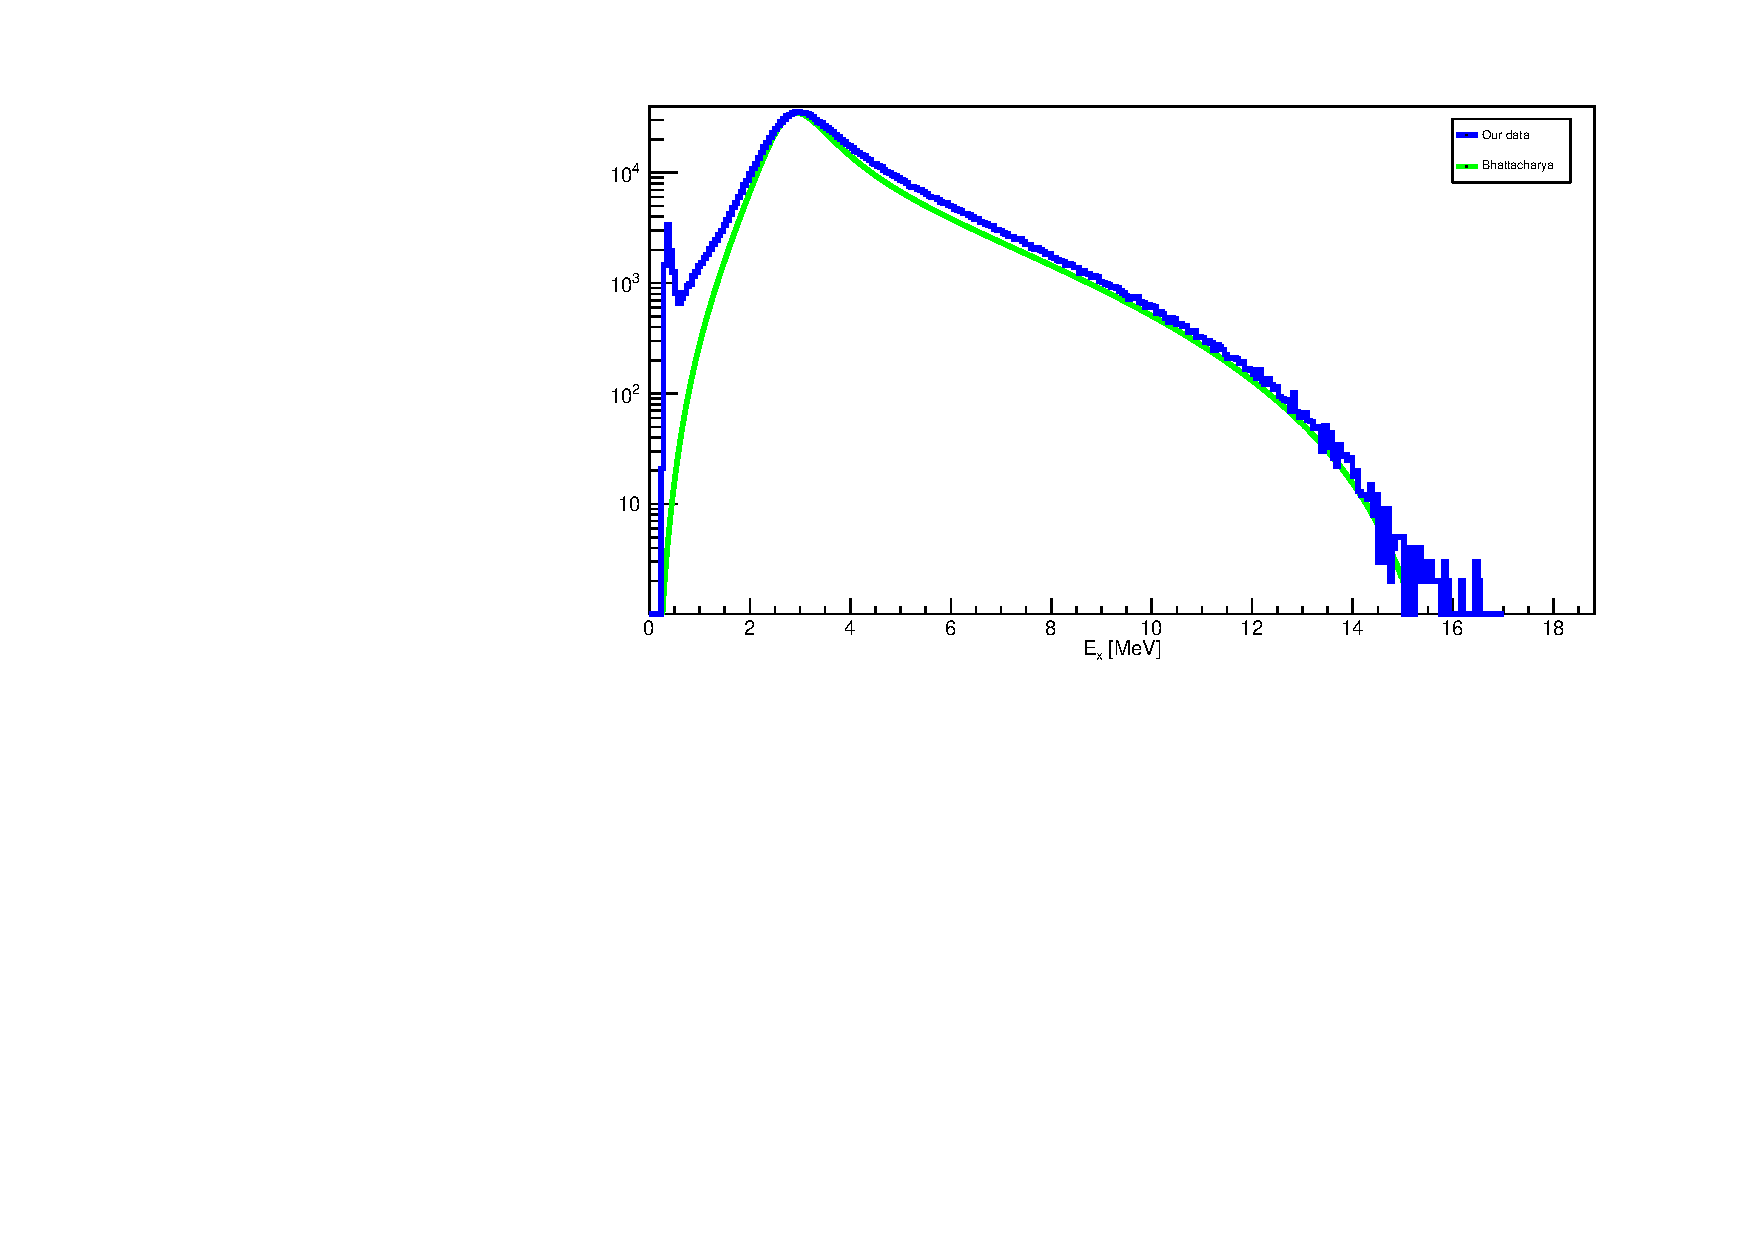
\includegraphics[width=.8\columnwidth]{../figures/bataraCompare.pdf}
	
\end{frame}

\begin{frame}{Lepton rekyl - måske skip slide?}
	Forskel i energi mellem $\alpha_1$ og $\alpha_2$\\
	Indflydelse på $^8$Be peak\\
	Kan ikke undlades, som forslået af tidligere undersøgelser
	\begin{columns}
		\column[]{0.5\textwidth}\\
		\begin{figure}
			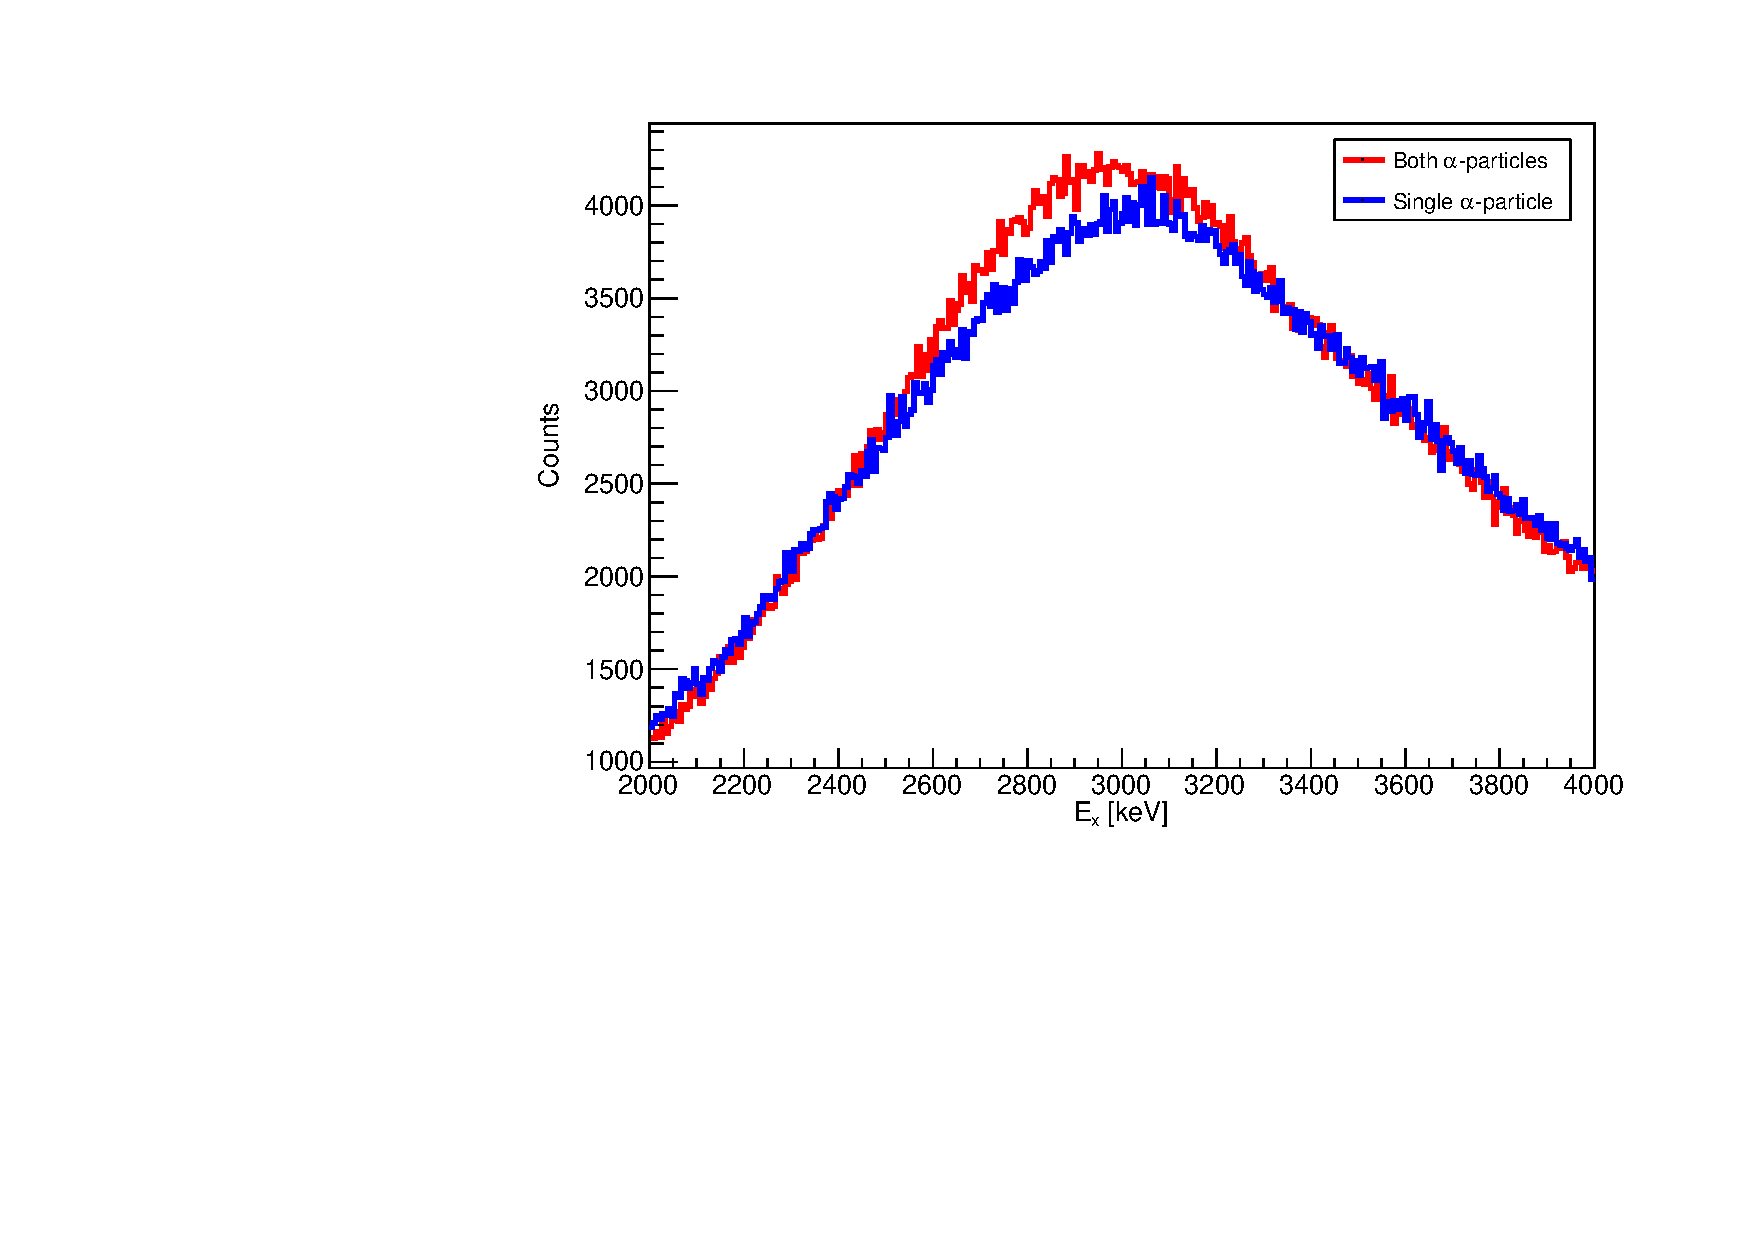
\includegraphics[width=\columnwidth]{../figures/recoil.pdf}
		\end{figure}
		\column[]{0.5\textwidth}\\
		\begin{figure}
			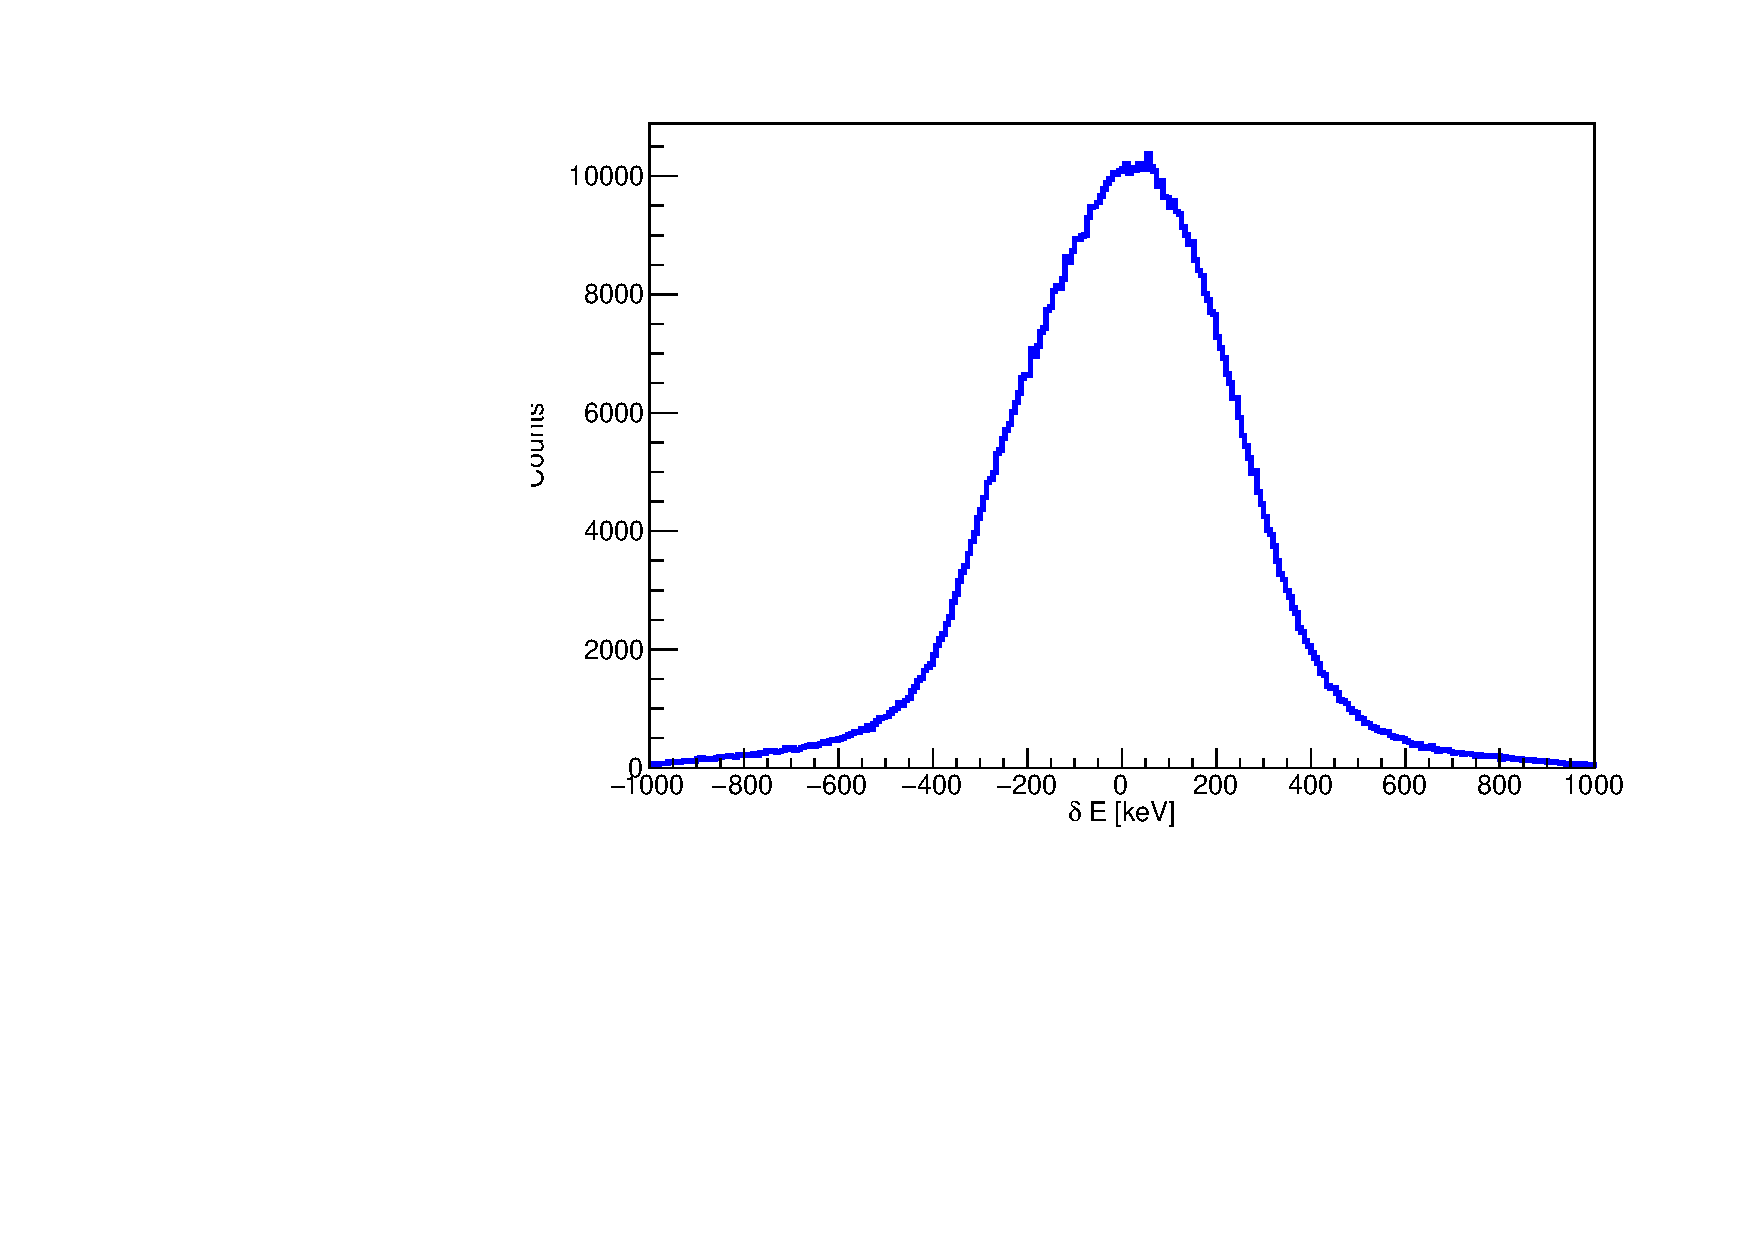
\includegraphics[width=\columnwidth]{../figures/recoilGauss.pdf}
		\end{figure}
	\end{columns}
\end{frame}

\begin{frame}{Vinkel korrelationer mellem \al\ og \be}
\begin{columns}
	\column{0.4\textwidth}
	\begin{itemize}
		\onslide<1->{\item Vinkel mellem $\alpha_1$ og \be\\}
		\onslide<2->{\item Vinkel mellem $\alpha_2$ og \be\\}
		\onslide<3->{\item Giver komplet billede sammenlagt}
		%\onslide<4->{\item Sammenligning med setup effektivitet}
	\end{itemize}
	\column{0.6\textwidth}
	\begin{overprint}
	\onslide<1>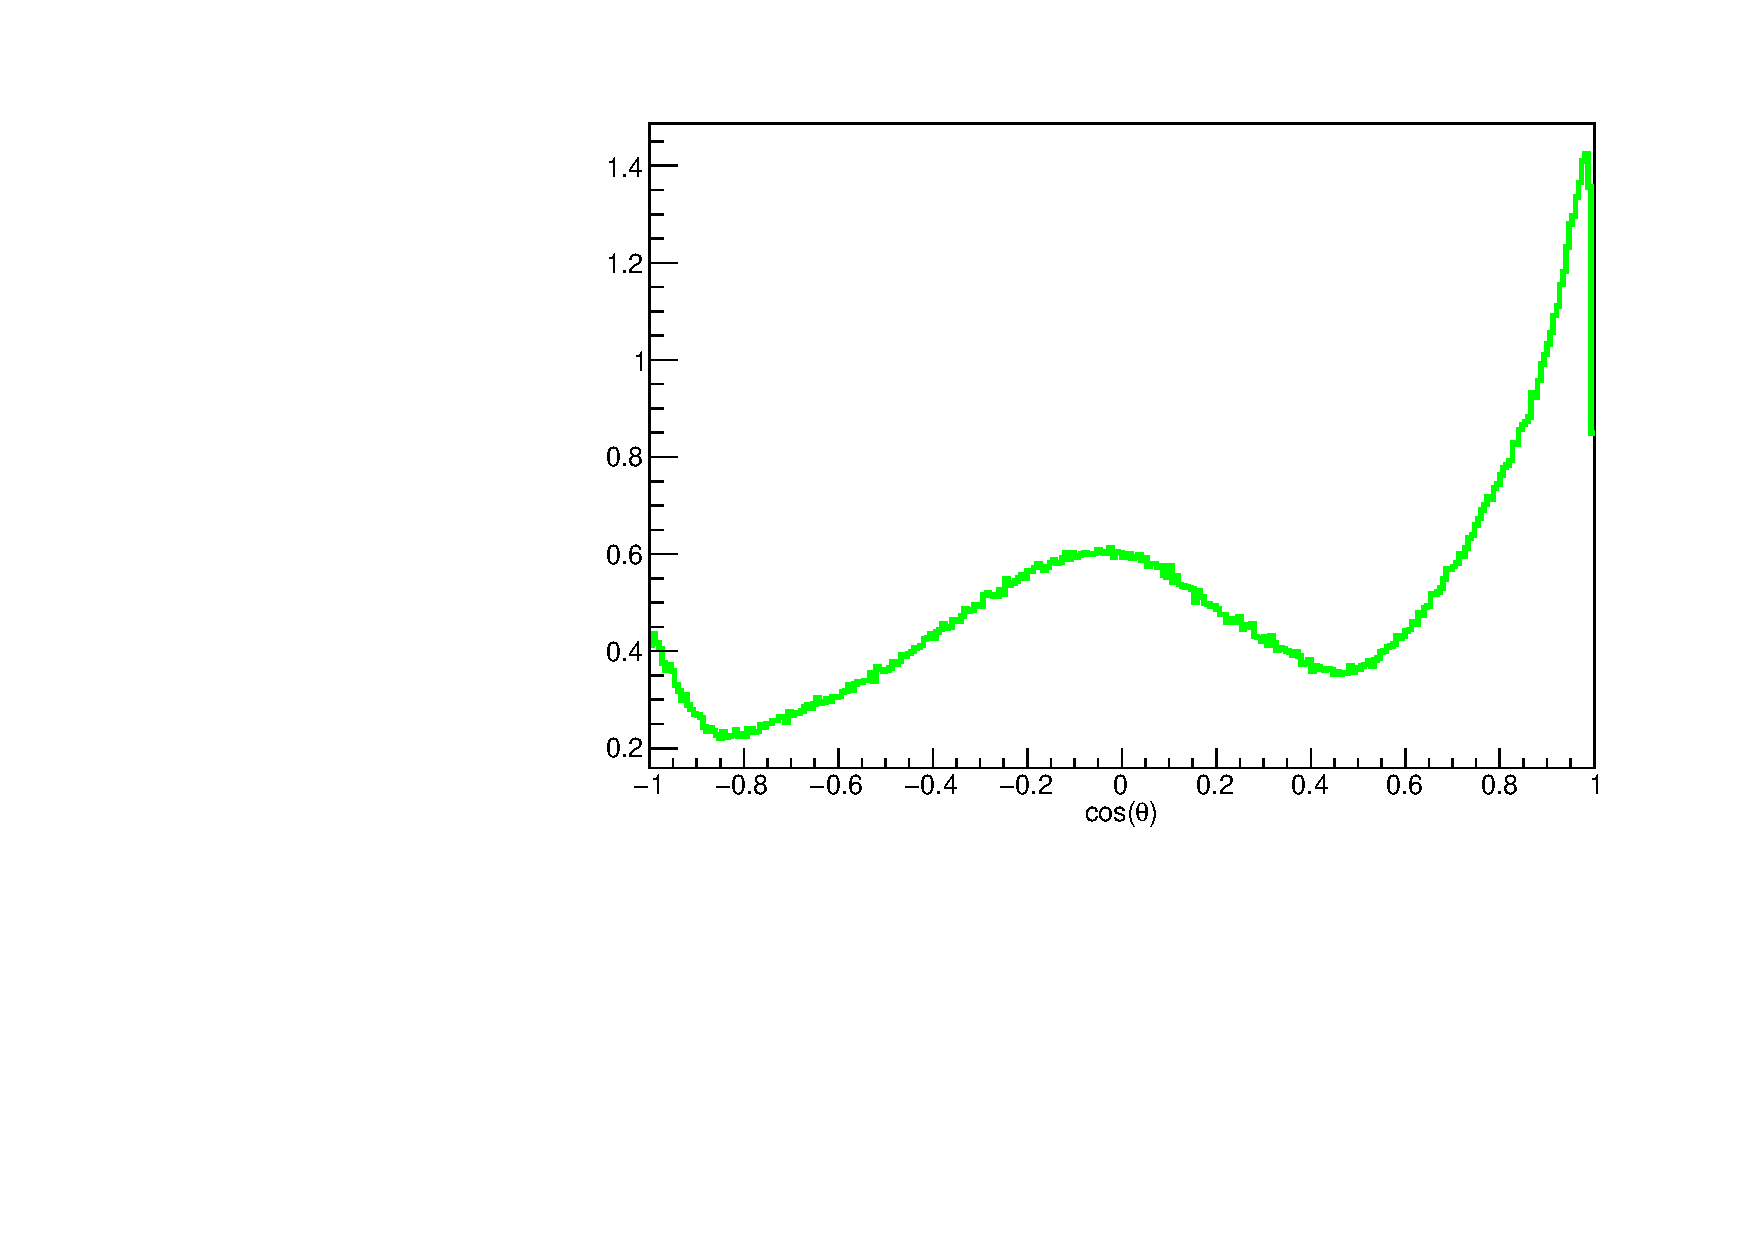
\includegraphics[width=\columnwidth]{../figures/justAl1.pdf}
	\onslide<2>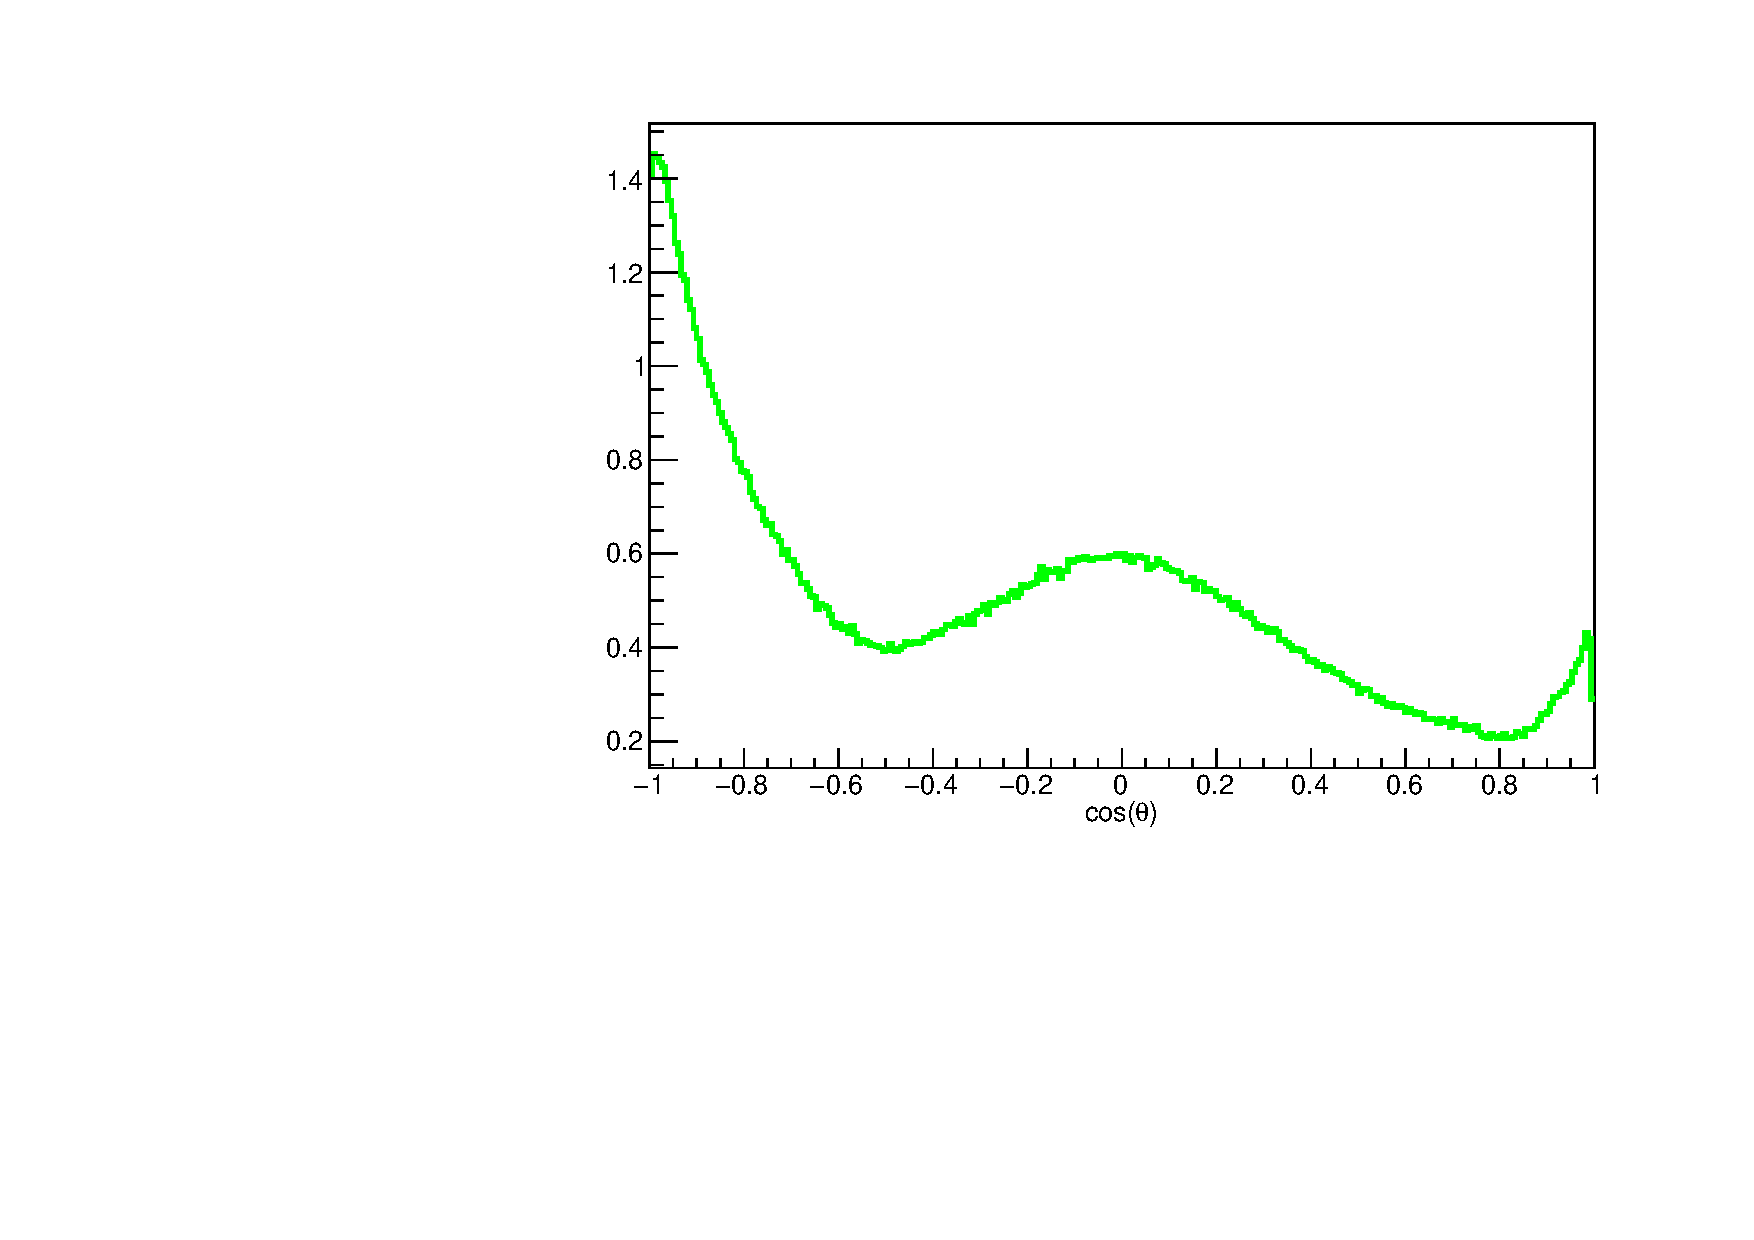
\includegraphics[width=\columnwidth]{../figures/justAl2.pdf}
	\onslide<3>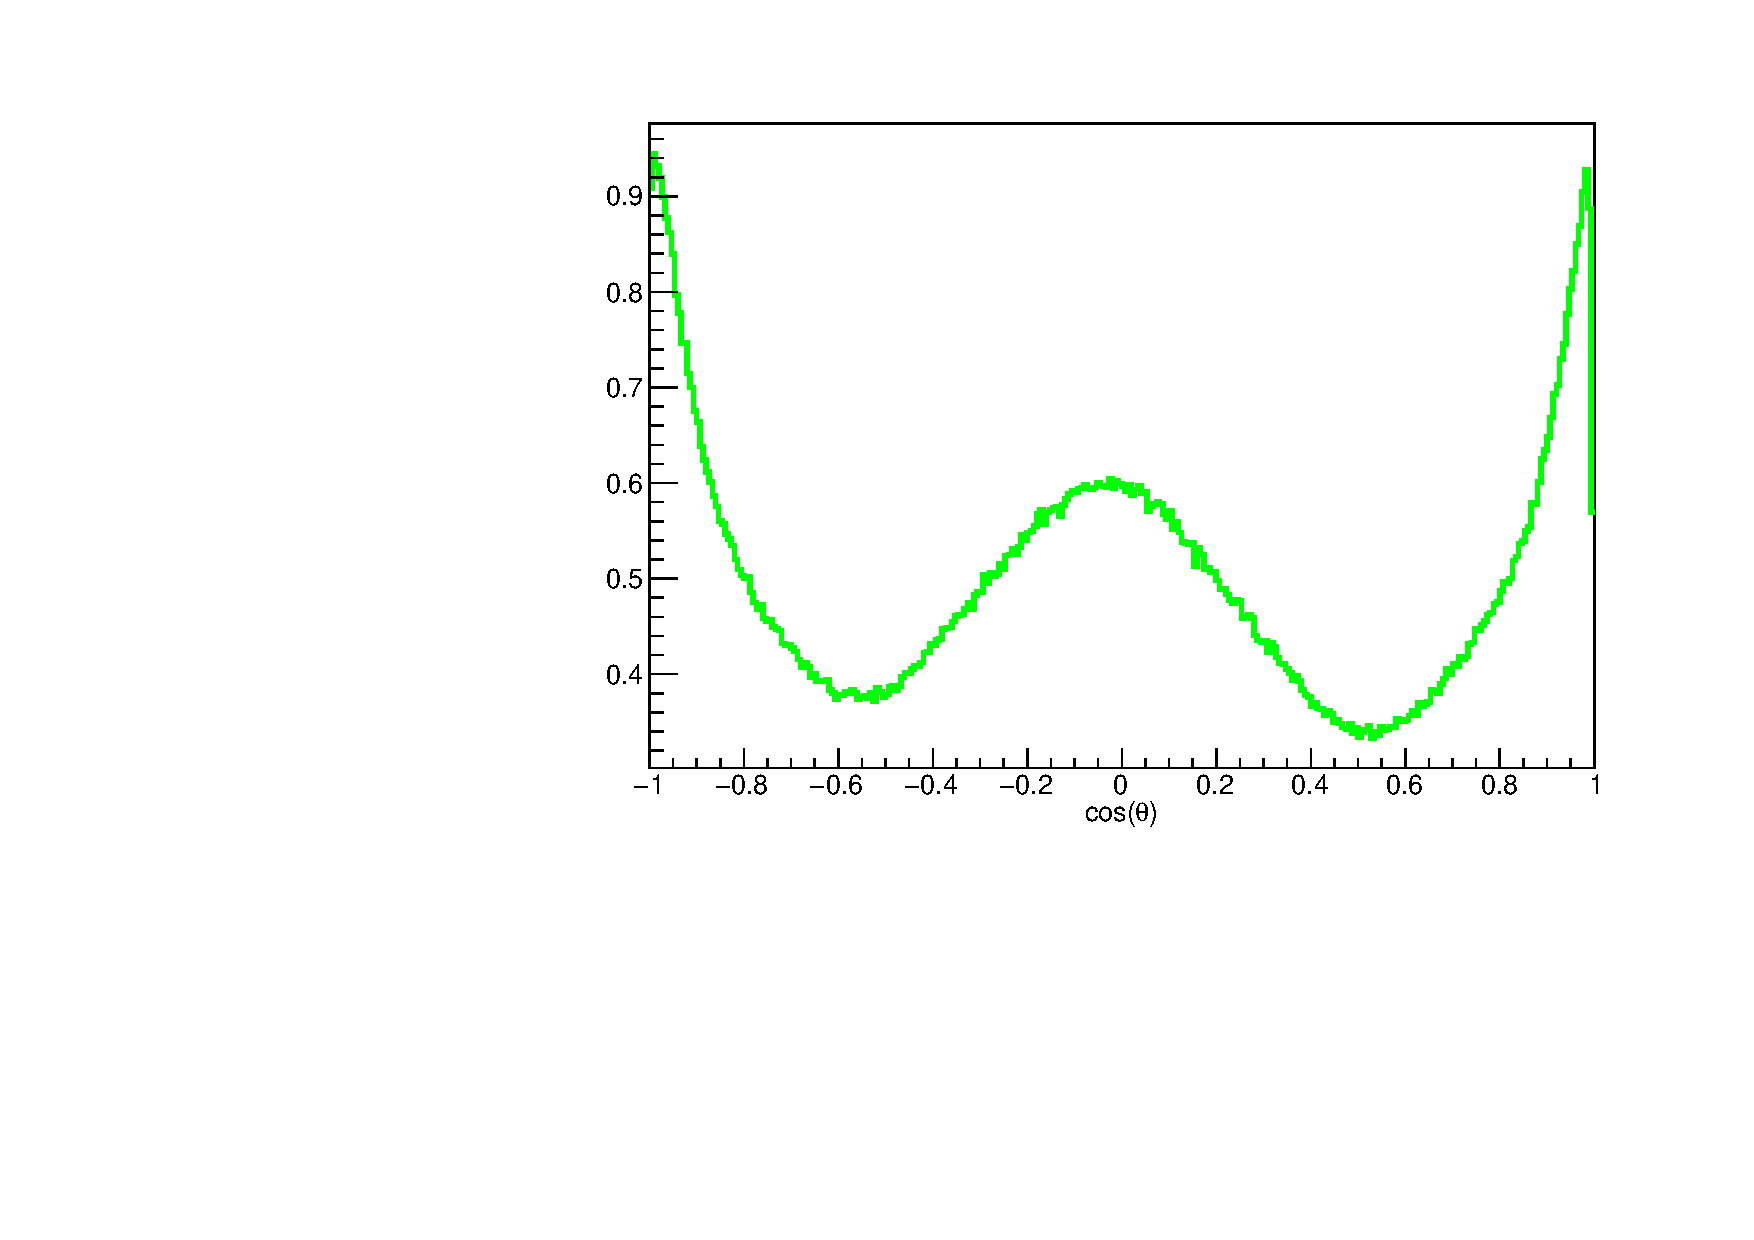
\includegraphics[width=\columnwidth]{../figures/justData.pdf}
	%\onslide<4->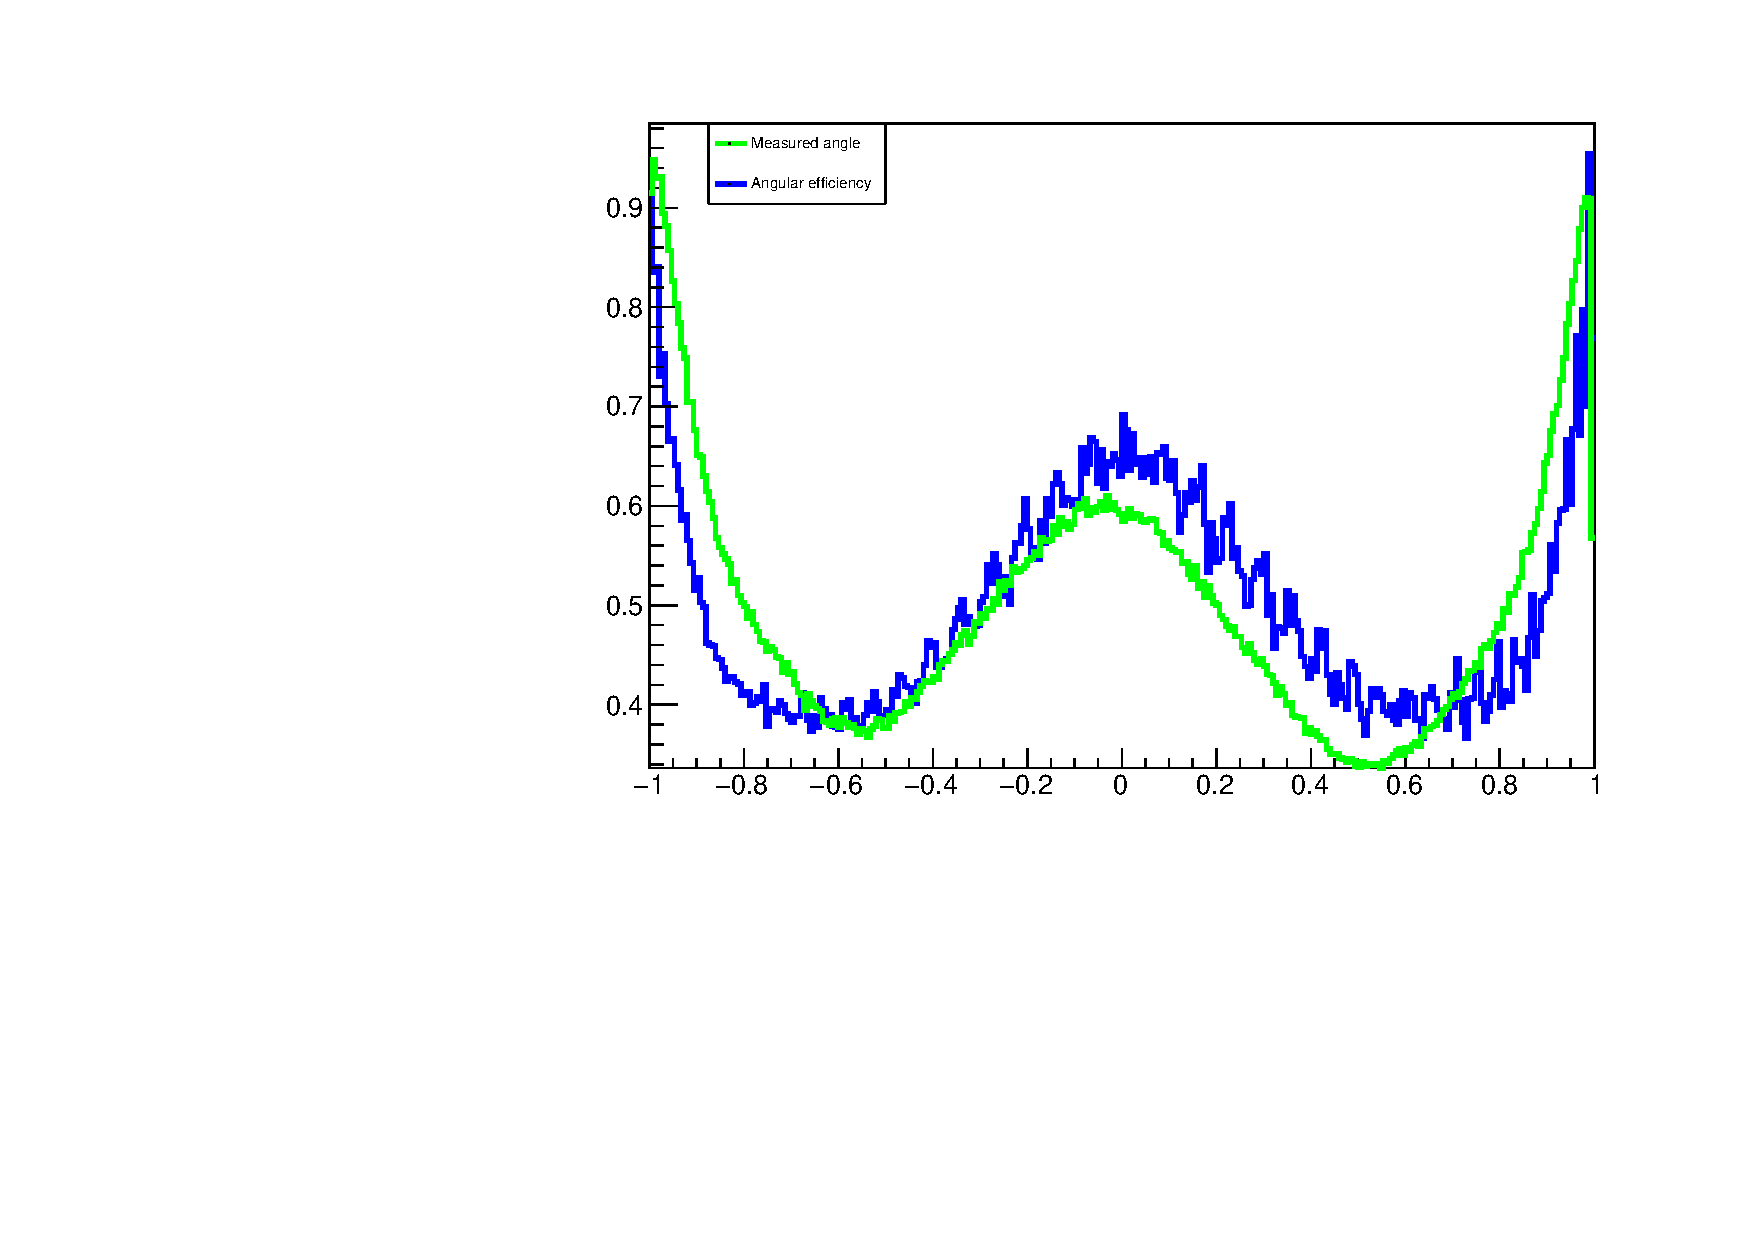
\includegraphics[width=\columnwidth]{../figures/betaAngles/betaAngle.pdf}
	\end{overprint}	
\end{columns}
\end{frame}

\begin{frame}{Setup effektivitet}
	\begin{columns}
		\column[]{.6\textwidth}
		\begin{itemize}
			\onslide<1->{\item Setup har større sandsynlighed for at måle nogle individuelle vinkler\\}
			\onslide<2->{\item Der vil altid være \textcolor{blue}{$0\degree$} mellem en pixel og sig selv\\}
			\onslide<3->{\item Ofte en pixel \textcolor{mypurple}{$90\degree$} eller \textcolor{mypurple}{$180\degree$} fra en given pixel\\}
			\onslide<4->{\item Ikke altid en pixel \textcolor{red}{$45\degree$} eller \textcolor{red}{$135\degree$} fra en pixel}
		\end{itemize}
		
		\column[]{.4\textwidth}
		\begin{overprint}
			\onslide<2>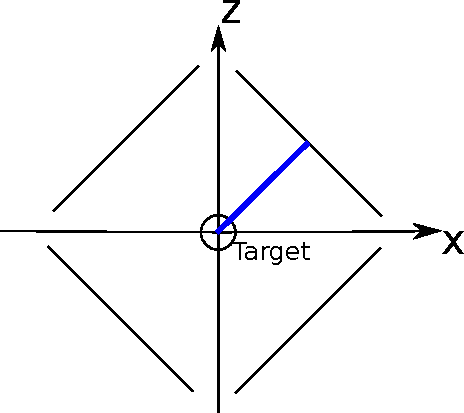
\includegraphics[width=\columnwidth]{../figures/showAngles/opstilling_show_angles_1.pdf}
			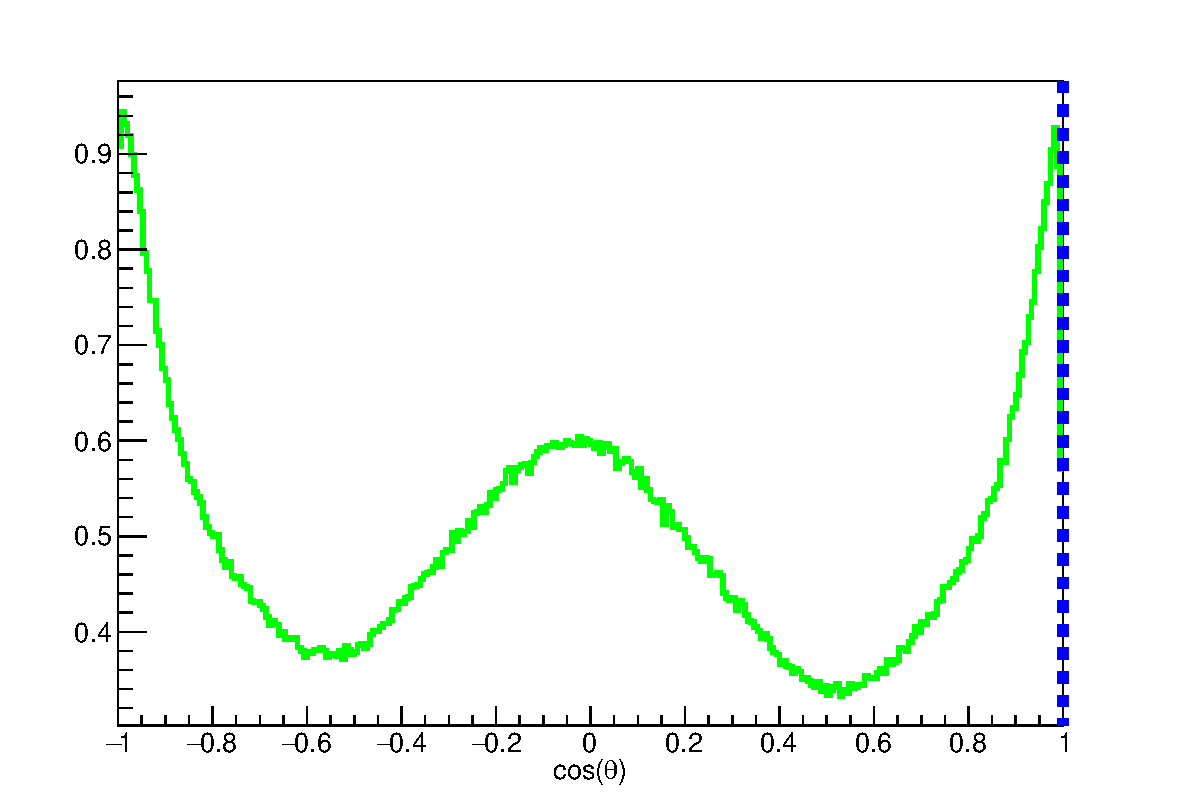
\includegraphics[width=\columnwidth]{../figures/showAngles/data_1.pdf}
			\onslide<3>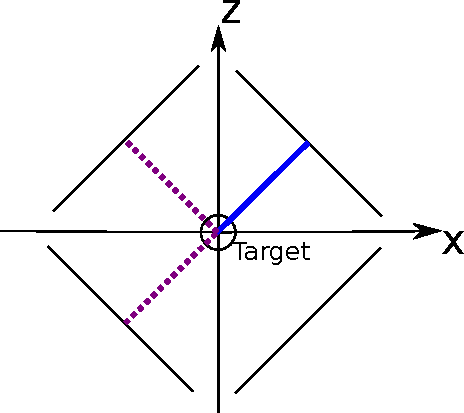
\includegraphics[width=\columnwidth]{../figures/showAngles/opstilling_show_angles_2.pdf}
			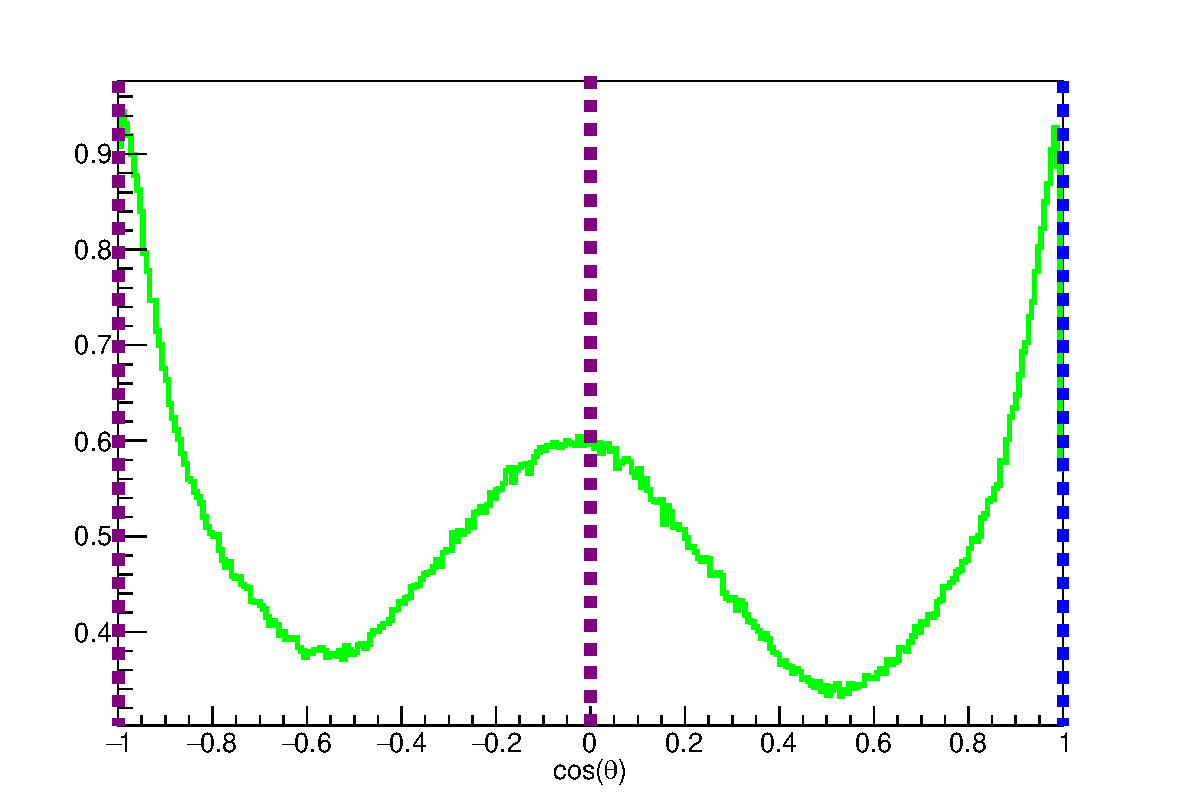
\includegraphics[width=\columnwidth]{../figures/showAngles/data_2.pdf}
			\onslide<4->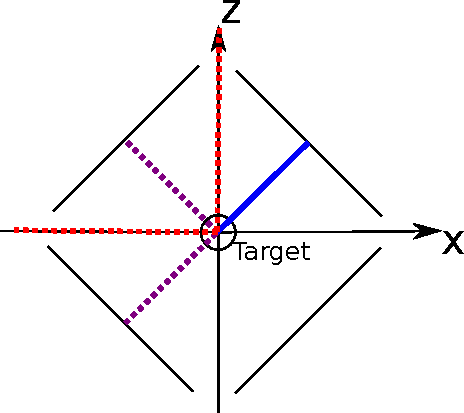
\includegraphics[width=\columnwidth]{../figures/showAngles/opstilling_show_angles_3.pdf}
			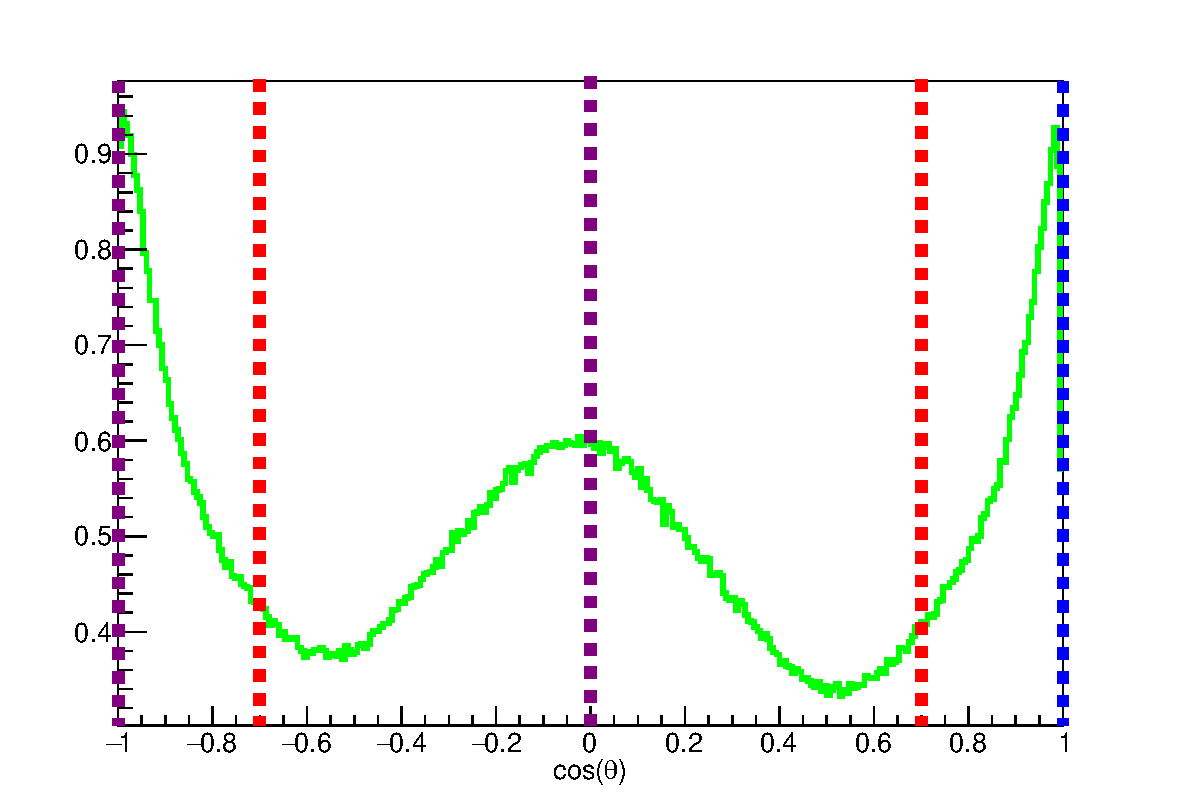
\includegraphics[width=\columnwidth]{../figures/showAngles/data_3.pdf}
		\end{overprint}
	\end{columns}
\end{frame}

\begin{frame}{Setup effektivitet}
	\begin{itemize}
		\onslide<1->{\item Udregn den forventede vinkelfordeling}
		\onslide<2->{\item Vinklen mellem en pixel $i$ i en hvilken som helst detektor, og en anden pixel $j$ i en given detektor}
	\end{itemize}
	\begin{columns}
		\column[]{.5\textwidth}
		\onslide<3->
		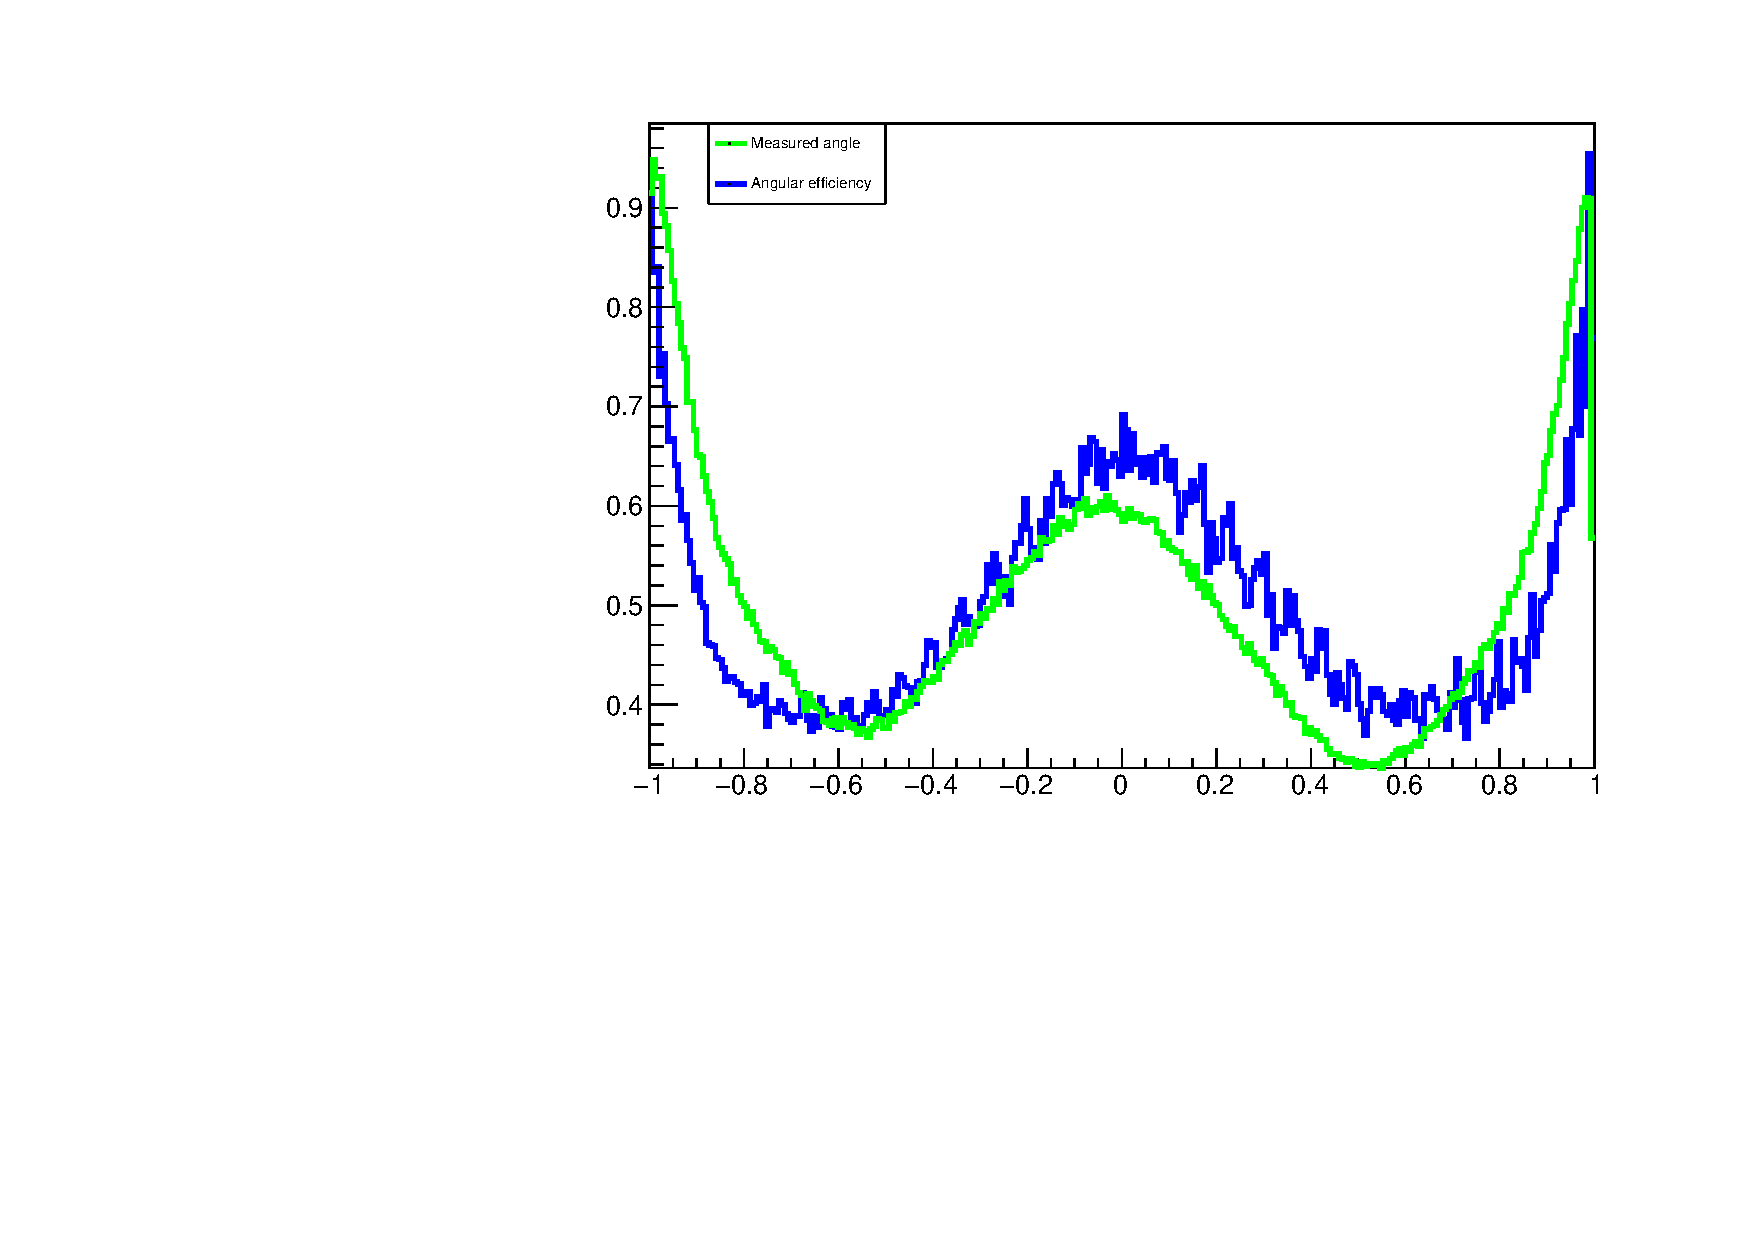
\includegraphics[width=\columnwidth]{../figures/betaAngles/betaAngle.pdf}
		\column[]{.5\textwidth}
		\onslide<4->
		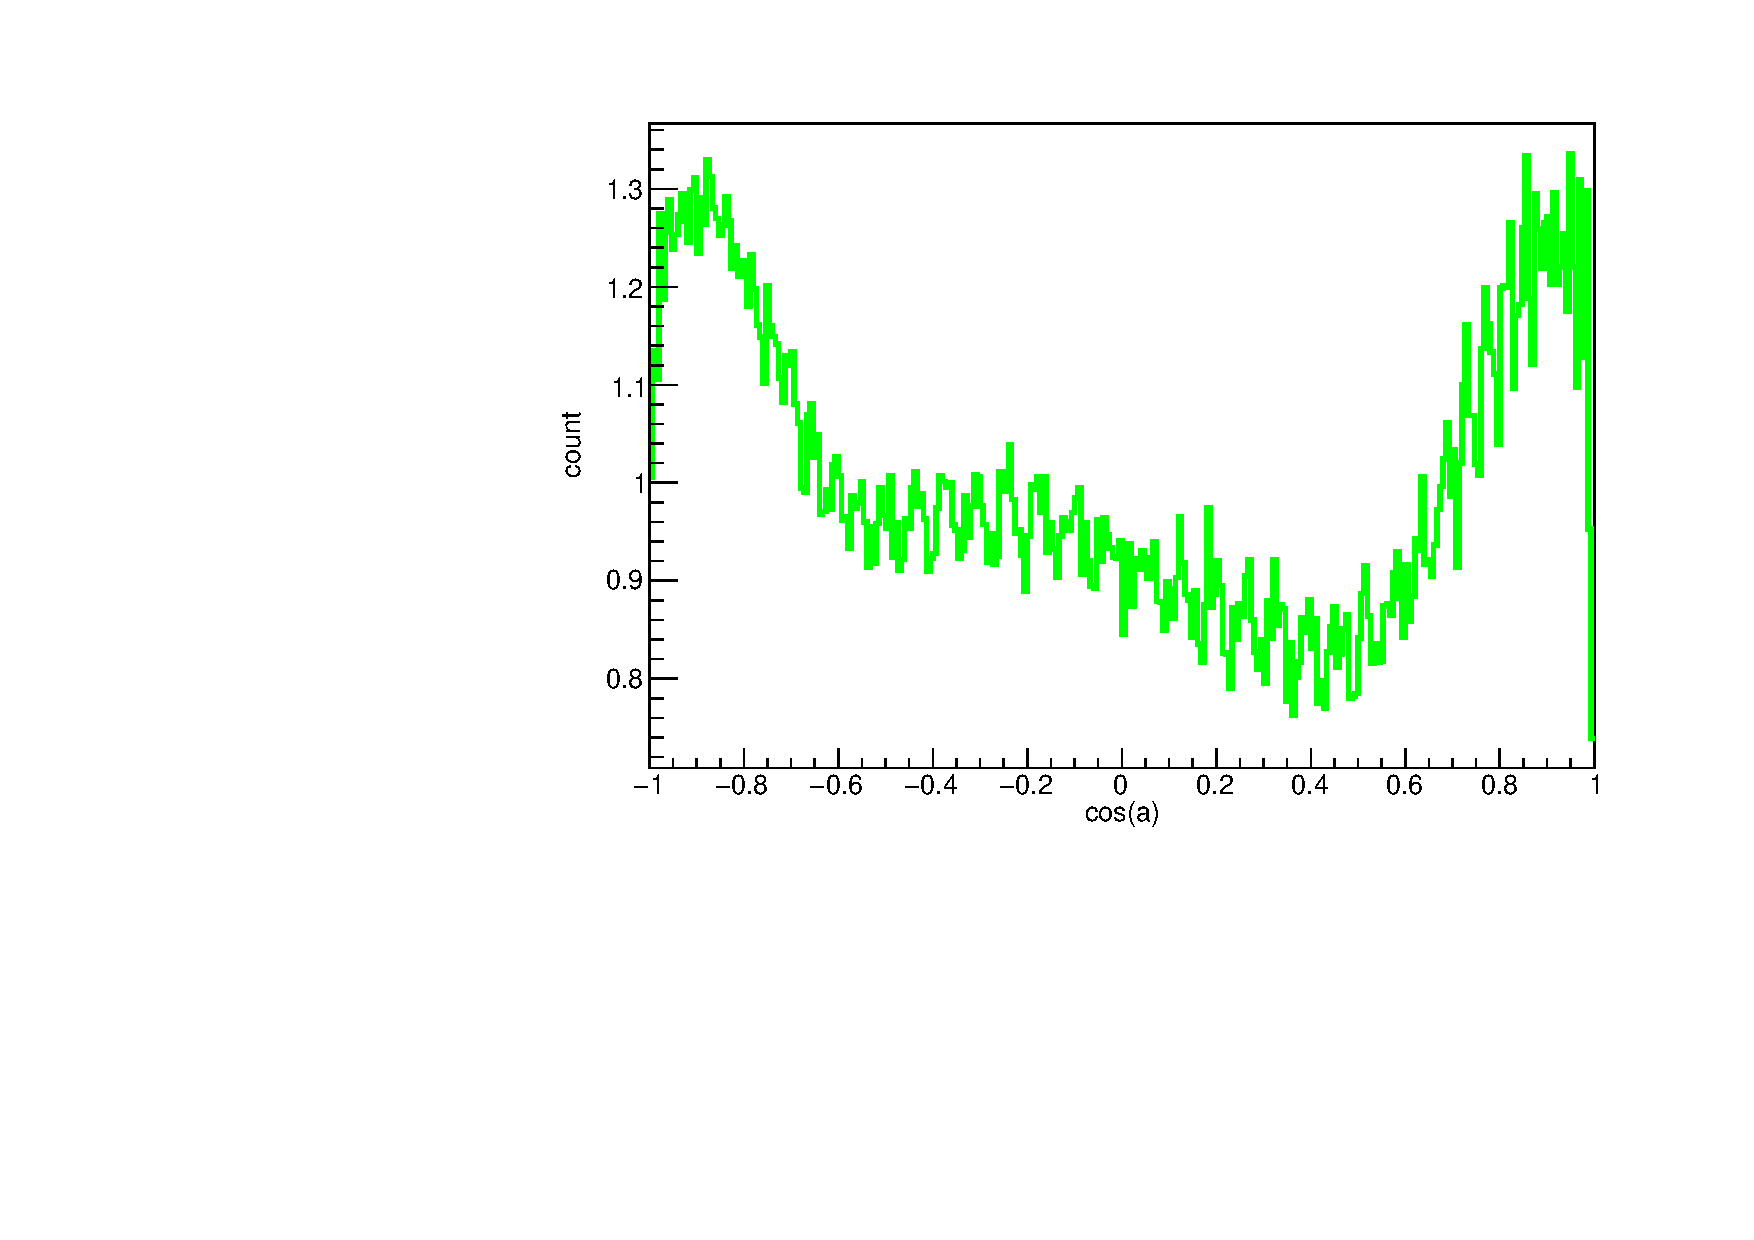
\includegraphics[width=\columnwidth]{../figures/betaAngles/dataDivEff.pdf}
	\end{columns}
\end{frame}

\begin{frame}{Geometriske forskydninger}
	Mulige fejlkilder
	\begin{itemize}
		\onslide<2->{\item Beam rammer ikke lige i center af target}
		\onslide<3->{\item Detektorerne står anderledes end antaget}
		\onslide<4->{\item Target-holderen skygger for data}
		\onslide<5->{\item Døde strips}
	\end{itemize}
\end{frame}

\begin{frame}{Center forskydning}
	\begin{itemize}
		\onslide<2->{\item Ryk på hvor beam rammer i effektivitetsudregningen }
		\onslide<3->{\item Se hvad der passer bedst}
		\onslide<4->{\item Alle 3 dimensioner der kan være forkerte}
		\onslide<5->{\item Bedste match fundet ved at rykke center $(-3, -3, 0)$ (mm)}
	\end{itemize}
\begin{columns}
	\column[]{.5\textwidth}
	\begin{overprint}
		\onslide<3-4>
		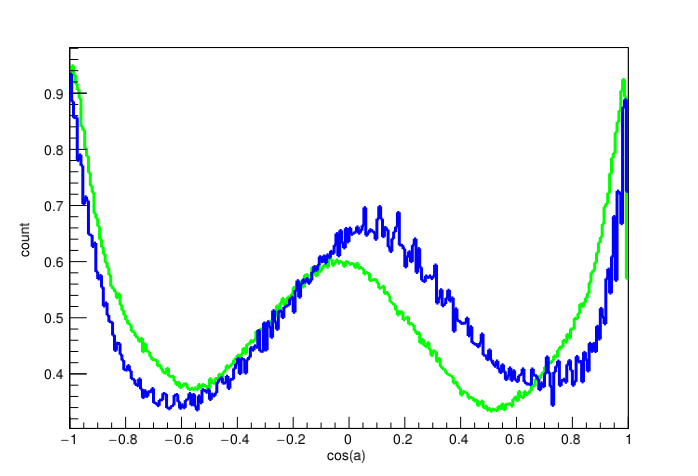
\includegraphics[width=\columnwidth]{../figures/centerCorrections/try33-3.png}
		\onslide<5->
		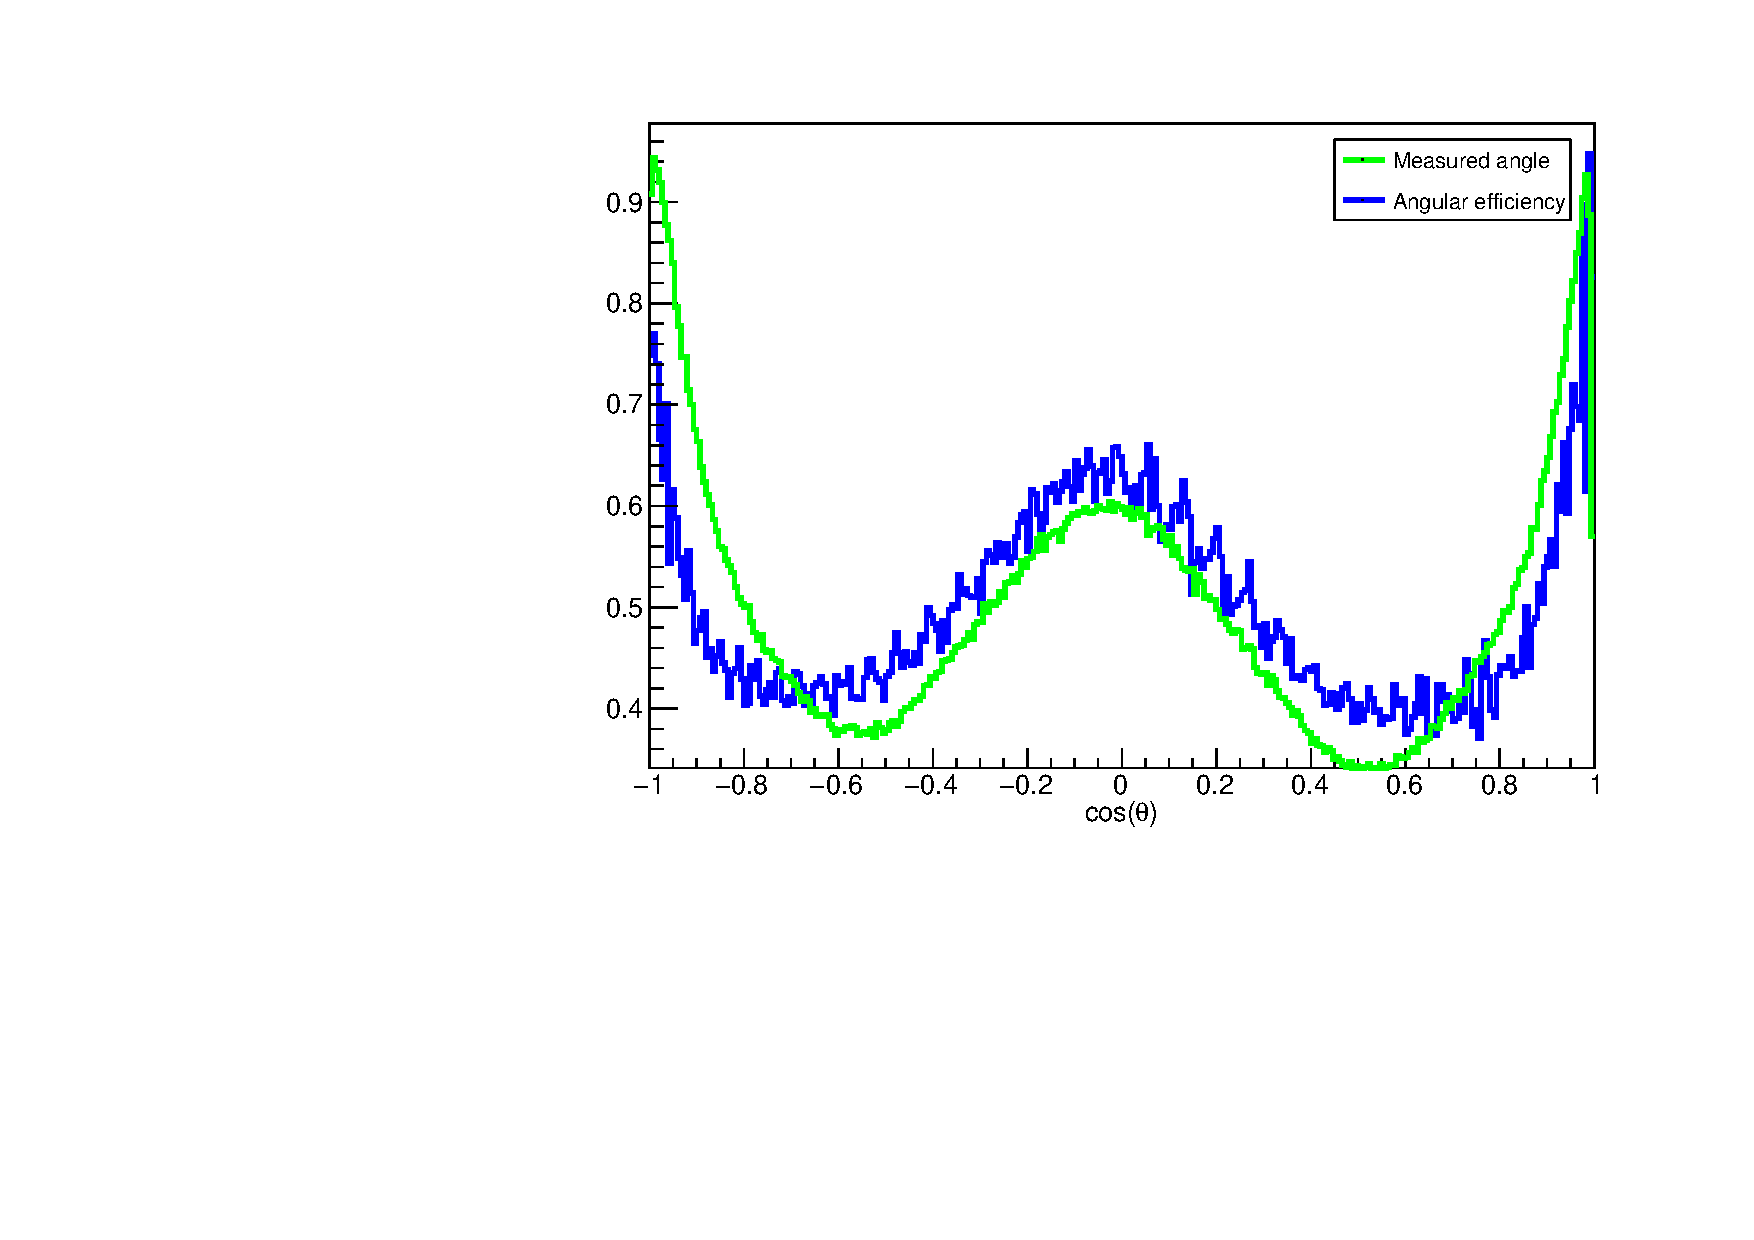
\includegraphics[width=\columnwidth]{../figures/betaAngles/centerCorrectedAndData.pdf}
	\end{overprint}
	
	\column[]{.5\textwidth}
	\onslide<5->
	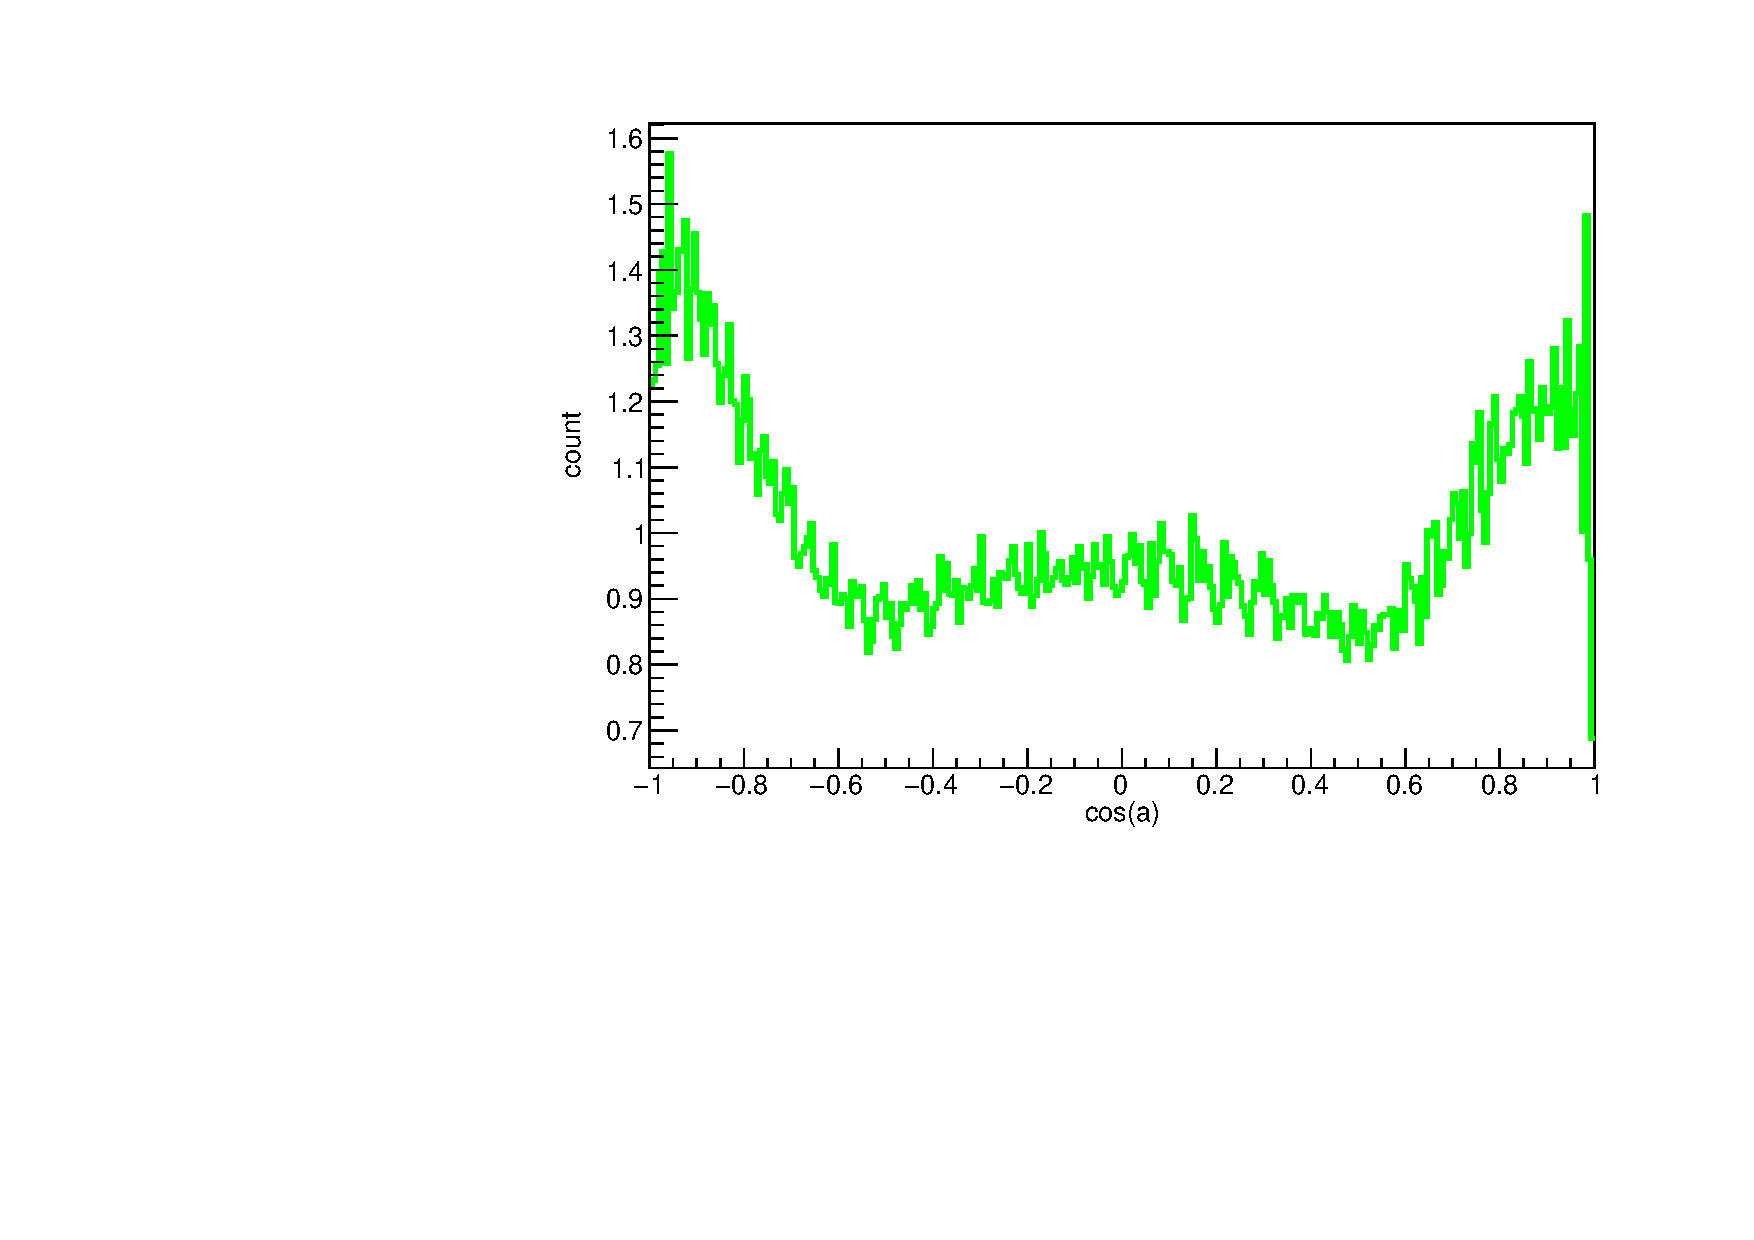
\includegraphics[width=\columnwidth]{../figures/betaAngles/dataDivEffCenterCorrected.pdf}
\end{columns}
\end{frame}

\begin{frame}{Døde strips, skygger og placering}
	\begin{itemize}
		\item Targetholderen kaster skygge på øvre og nedre detektor
		\item Døde strips 
		\item Koncentration af hits forskellig fra hvad vi forventer
	\end{itemize}
	\begin{columns}
		\column[]{.5\textwidth}
		\centering
		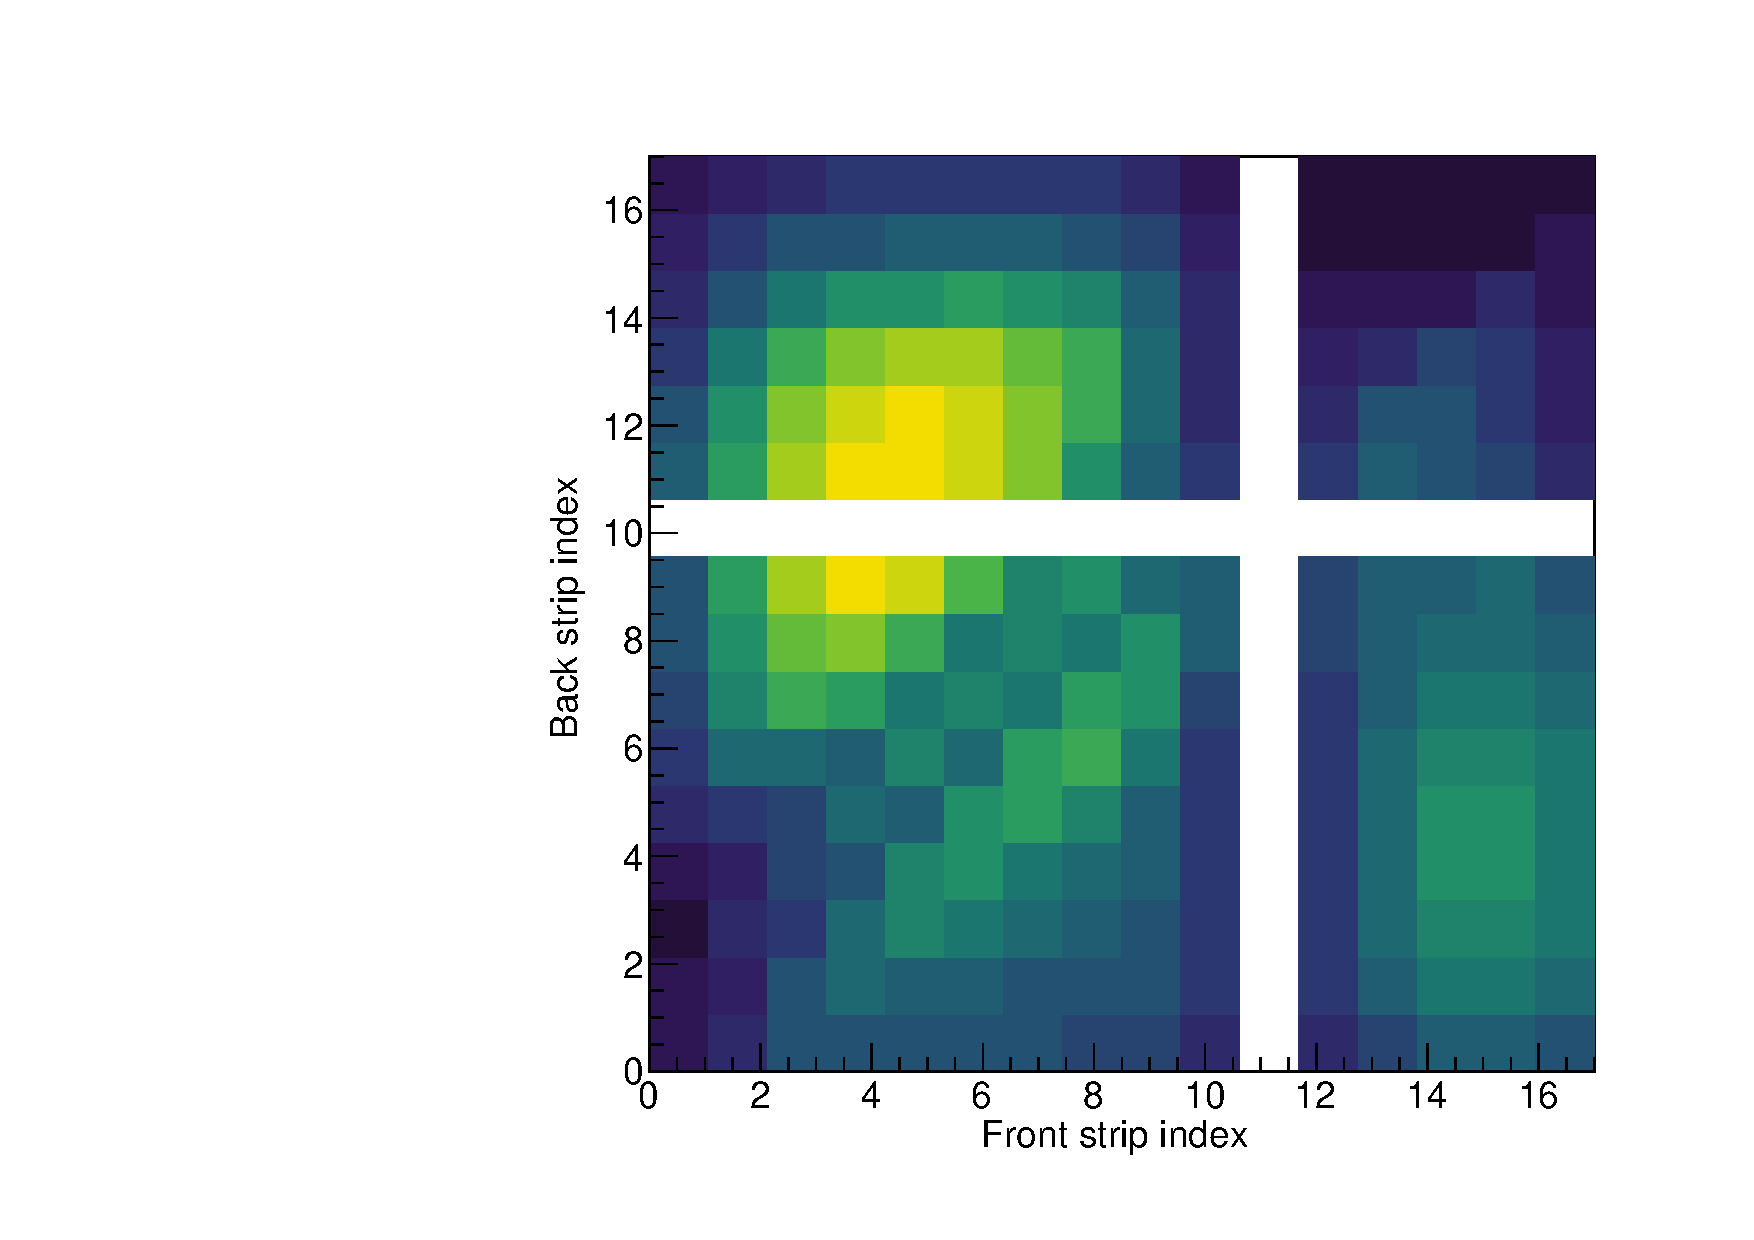
\includegraphics[width=\columnwidth]{../figures/mexihatDet4.pdf}
		\tiny Data
		\column[]{.5\textwidth}
		\centering
		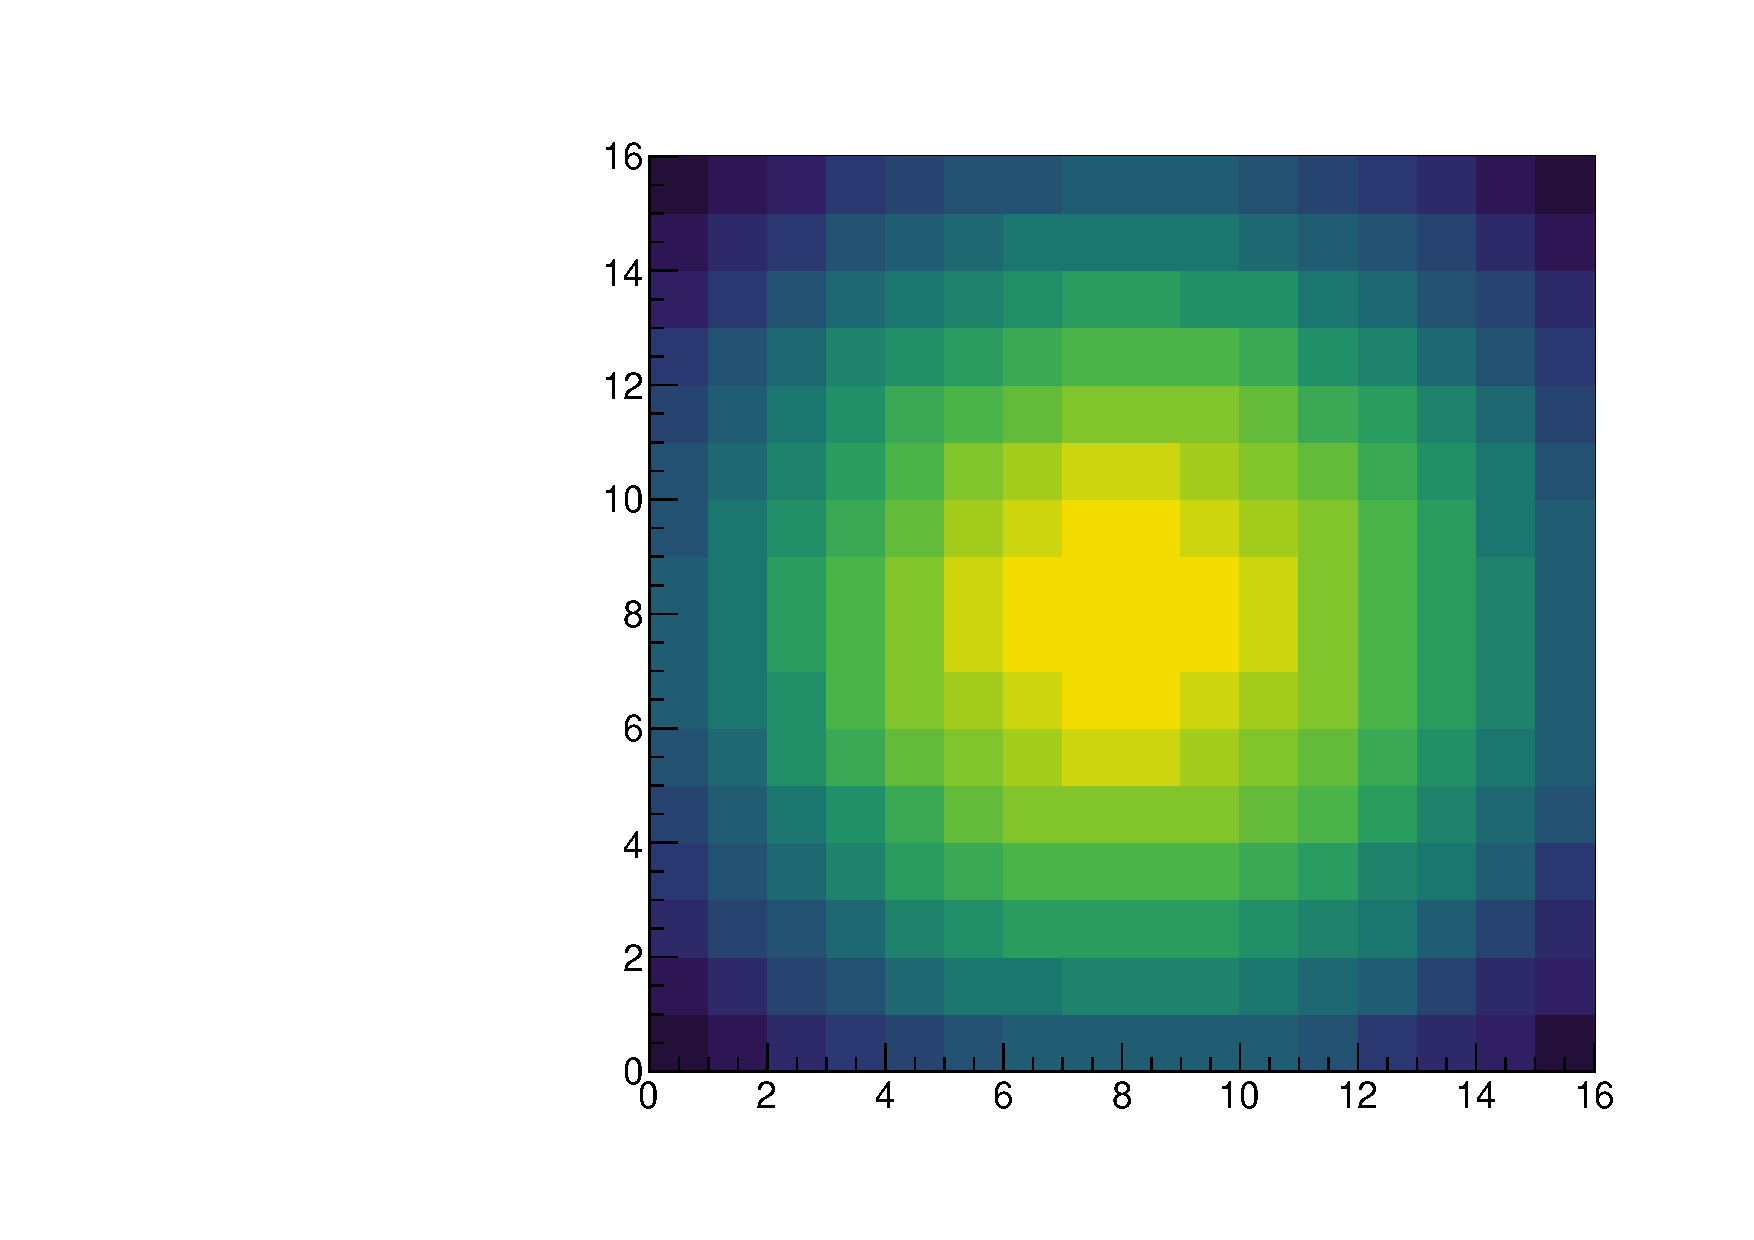
\includegraphics[width=\columnwidth]{../figures/mexihatDet4Theory.pdf}
		\tiny Udregnet effektivitet
	\end{columns}
\end{frame}

\end{document}